%% FEUP THESIS STYLE for LaTeX2e
%% how to use feupteses (portuguese version)
%%
%% FEUP, JCL & JCF, 31 Jul 2012
%%
%% PLEASE send improvements to jlopes at fe.up.pt and to jcf at fe.up.pt
%%

%%========================================
%% Commands: pdflatex tese
%%           bibtex tese
%%           makeindex tese (only if creating an index)
%%           pdflatex tese
%% Alternative:
%%          latexmk -pdf tese.tex
%%========================================

\documentclass[11pt,a4paper,twoside,openright]{report}

%% For iso-8859-1 (latin1), comment next line and uncomment the second line
\usepackage[utf8]{inputenc}

%\usepackage[latin1]{inputenc}

%% Portuguese version

%% MIEIC options
%\usepackage[portugues,mieic]{feupteses}
%\usepackage[portugues,mieic,juri]{feupteses}
%\usepackage[portugues,mieic,final]{feupteses}
%\usepackage[portugues,mieic,final,onpaper]{feupteses}

%% MIEEC options
%\usepackage[portugues,mieec]{feupteses}
%\usepackage[portugues,mieec,juri]{feupteses}
%\usepackage[portugues,mieec,final]{feupteses}
%\usepackage[portugues,mieec,final,onpaper]{feupteses}

%% For other degrees
\usepackage[mieec,juri]{feupteses} % you must define the degree bellow

%% Options: 
%% - portugues: titles, etc in portuguese
%% - onpaper: links are not shown (for paper versions)
%% - backrefs: include back references from bibliography to citation place

%% Uncomment to create an index (at the end of the document)
%\makeindex

%% Path to the figures directory
%% TIP: use folder ``figures'' to keep all your figures
\graphicspath{{figures/}}

%%----------------------------------------
%% TIP: if you want to define more macros, use an external file to keep them
%some macro definitions

% format
\newcommand{\class}[1]{{\normalfont\slshape #1\/}}

% entities
\newcommand{\Feup}{Faculdade de Engenharia da Universidade do Porto}


\newcommand{\svg}{\class{SVG}}
\newcommand{\scada}{\class{SCADA}}
\newcommand{\scadadms}{\class{SCADA/DMS}}

\usepackage{mypackages}


\addbibresource{myrefs.bib}
%%----------------------------------------

%%========================================
%% Start of document
%%========================================
\begin{document}

%%----------------------------------------
%% Information about the work
%%----------------------------------------
\title{Event Driven Publish/Subscribe Consumer Group Autoscaling}
\author{Diogo Landau}

%% Comment next line if not necessary for degree name
\degree{Mestrado Integrado em Engenharia Eletrotécnica e Computadores}

%% Uncomment next line for date of submission
%\thesisdate{31 de julho de 2008}

%% Comment next line for copyright text if not used
%\copyrightnotice{Diogo Landau, 2021/2022}

\supervisor{Supervisor}{Jorge Barbosa}

%% Uncomment next line if necessary
%\supervisor{Co-orientador}{Nome de Outro Orientador}

%% Uncomment committee stuff in the final version if used
%\committeetext{Aprovado em provas públicas pelo Júri:}
%\committeemember{Presidente}{Nome do presidente do júri}
%\committeemember{Arguente}{Nome do arguente do júri}
%\committeemember{Vogal}{Nome do vogal do júri}

%% Uncomment signature line in the final on paper version if used
%\signature

%% Specify cover logo (in folder ``figures'')
\logo{uporto-feup.pdf}
 
%% Uncomment next line for additional text below the author's name (front page)
%\additionalfronttext{Preparação da Dissertação}

%%----------------------------------------
%% Preliminary materials
%%----------------------------------------

% remove unnecessary \include{} commands
\begin{Prolog}
  \chapter*{Resumo}
%\addcontentsline{toc}{chapter}{Resumo}

Este documento ilustra o formato a usar em dissertações na \Feup.
São dados exemplos de margens, cabeçalhos, títulos, paginação, estilos
de índices, etc. 
São ainda dados exemplos de formatação de citações, figuras e tabelas,
equações, referências cruzadas, lista de referências e índices.
Este documento não pretende exemplificar conteúdos a usar. 
É usado o \emph{Loren Ipsum} para preencher a dissertação.

Lorem ipsum dolor sit amet, consectetuer adipiscing elit. Etiam vitae
quam sed mauris auctor porttitor. Mauris porta sem vitae arcu sagittis
facilisis. Proin sodales risus sit amet arcu. Quisque eu pede eu elit
pulvinar porttitor. Maecenas dignissim tincidunt dui. Pellentesque
habitant morbi tristique senectus et netus et malesuada fames ac
turpis egestas. Donec non augue sit amet nulla gravida
rutrum. Vestibulum ante ipsum primis in faucibus orci luctus et
ultrices posuere cubilia Curae; Nunc at nunc. Etiam egestas. 

Donec malesuada pede eget nunc. Fusce porttitor felis eget mi mattis
vestibulum. Pellentesque faucibus. Cras adipiscing dolor quis
mi. Quisque sagittis, justo sed dapibus pharetra, lectus velit
tincidunt eros, ac fermentum nulla velit vel sapien. Vestibulum sem
mauris, hendrerit non, feugiat ac, varius ornare, lectus. Praesent
urna tellus, euismod in, hendrerit sit amet, pretium vitae,
nisi. Proin nisl sem, ultrices eget, faucibus a, feugiat non,
purus. Etiam mi tortor, convallis quis, pharetra ut, consectetuer eu,
orci. Vivamus aliquet. Aenean mollis fringilla erat. Vivamus mollis,
purus at pellentesque faucibus, sapien lorem eleifend quam, mollis
luctus mi purus in dui. Maecenas volutpat mauris eu lectus. Morbi vel
risus et dolor bibendum malesuada. Donec feugiat tristique erat. Nam
porta auctor mi. Nulla purus. Nam aliquam. 


\chapter*{Abstract}
%\addcontentsline{toc}{chapter}{Abstract}

The increase in photovoltaic power plants has led to the need for effective
methods for detecting and addressing component faults, which can have
significant economic impacts. In this work, we will explore the current state of
fault detection and state estimation tools in the field of PV systems, with a
focus on understanding how these tools work and identifying their strengths and
limitations. We will also propose improvements to existing approaches or develop
a novel approach to address this issue. By examining the most successful tools
to date and offering new solutions, we aim to help PV plant operators improve
the reliability and efficiency of their systems. % the abstract
  \chapter*{Agradecimentos}
%\addcontentsline{toc}{chapter}{Agradecimentos}

Aliquam id dui. Nulla facilisi. Nullam ligula nunc, viverra a, iaculis
at, faucibus quis, sapien. Cum sociis natoque penatibus et magnis dis
parturient montes, nascetur ridiculus mus. Curabitur magna ligula,
ornare luctus, aliquam non, aliquet at, tortor. Donec iaculis nulla
sed eros. Sed felis. Nam lobortis libero. Pellentesque
odio. Suspendisse potenti. Morbi imperdiet rhoncus magna. Morbi
vestibulum interdum turpis. Pellentesque varius. Morbi nulla urna,
euismod in, molestie ac, placerat in, orci. 

Ut convallis. Suspendisse luctus pharetra sem. Sed sit amet mi in diam
luctus suscipit. Nulla facilisi. Integer commodo, turpis et semper
auctor, nisl ligula vestibulum erat, sed tempor lacus nibh at
turpis. Quisque vestibulum pulvinar justo. Class aptent taciti
sociosqu ad litora torquent per conubia nostra, per inceptos
himenaeos. Nam sed tellus vel tortor hendrerit pulvinar. Phasellus
eleifend, augue at mattis tincidunt, lorem lorem sodales arcu, id
volutpat risus est id neque. Phasellus egestas ante. Nam porttitor
justo sit amet urna. Suspendisse ligula nunc, mollis ac, elementum
non, venenatis ut, mauris. Mauris augue risus, tempus scelerisque,
rutrum quis, hendrerit at, nunc. Nulla posuere porta orci. Nulla dui. 

Fusce gravida placerat sem. Aenean ipsum diam, pharetra vitae, ornare
et, semper sit amet, nibh. Nam id tellus. Etiam ultrices. Praesent
gravida. Aliquam nec sapien. Morbi sagittis vulputate dolor. Donec
sapien lorem, laoreet egestas, pellentesque euismod, porta at,
sapien. Integer vitae lacus id dui convallis blandit. Mauris non
sem. Integer in velit eget lorem scelerisque vehicula. Etiam tincidunt
turpis ac nunc. Pellentesque a justo. Mauris faucibus quam id
eros. Cras pharetra. Fusce rutrum vulputate lorem. Cras pretium magna
in nisl. Integer ornare dui non pede. 

\vspace{10mm}
\flushleft{David Freire} % ? tem que ser o nome completo
  % the acknowledgments
  \cleardoublepage
\thispagestyle{plain}

\vspace*{8cm}

\begin{flushright}
   \textsl{``\\Genetic predispositions are only that: predispositions. \\
      It’s not a destiny written in stone. People have choices.''} \\
\vspace*{1.5cm}
            Dr. Jennifer Melfi, The Sopranos
\end{flushright}
    % initial quotation if desired
  \cleardoublepage
  \pdfbookmark[0]{Contents}{contents}
  \tableofcontents
  \cleardoublepage
  \pdfbookmark[0]{List of Figures}{figures}
  \listoffigures
  \cleardoublepage
  \pdfbookmark[0]{List of Tables}{tables}
  \listoftables
  \chapter*{Abreviaturas e Símbolos}
%\addcontentsline{toc}{chapter}{Abbreviations}
\chaptermark{ABREVIATURAS E SÍMBOLOS}

\begin{flushleft}
\begin{tabular}{l p{0.8\linewidth}}
PV      & Photovoltaic\\
DC      & Direct current\\
STC      & Standard Test Conditions\\
MCD      & Minimum Covariance Determinant\\
WWW      & \emph{World Wide Web}
\end{tabular}
\end{flushleft}

  % the list of abbreviations used
\end{Prolog}

%%----------------------------------------
%% Body
%%----------------------------------------

\StartBody

\chapter{Introduction} \label{chap:intro}

As a company becomes more reliant on the data it produces to drive its
decisions, data warehouses become core components for providing data for
analysis and reporting. To populate the data warehouse, one of the most common
procedures is the ETL (Extract, Transform and Load) process which involves:
extracting the data from multiple data sources; transforming the data; loading
the data into the appropriate format for consultation.

It is also well known that as companies become more data driven,
the challenges associated with dealing with large volumes of data becomes more
apparent as digital solutions start failing to respond, or are unable to respond
within appropriate time constraints. 

For this reason, a distributed architecture that resorts to microservices is a
common and efficient way to tackle the problem as it simplifies scaling based on
the system's needs, nullifies the single point of failure, and increases the
system's resilience. 

On the other hand, incorrectly implemented communication between microservices
can become a distributed solution's scalability bottleneck, as the microservice
components can become too coupled and increase the technical cost of making any
changes to the system.  This is where message brokers come in.  Instead of
having the components communicating with one another directly, the message
broker serves as an intermediary that asynchronously delivers the information
between components as it is requested by the interested parts. In short, the
message broker mediates the communication between data producers (entities that
send data to the broker) and data consumers (entities that request data from
the broker). 

\begin{figure}[htb!]
    \centering
    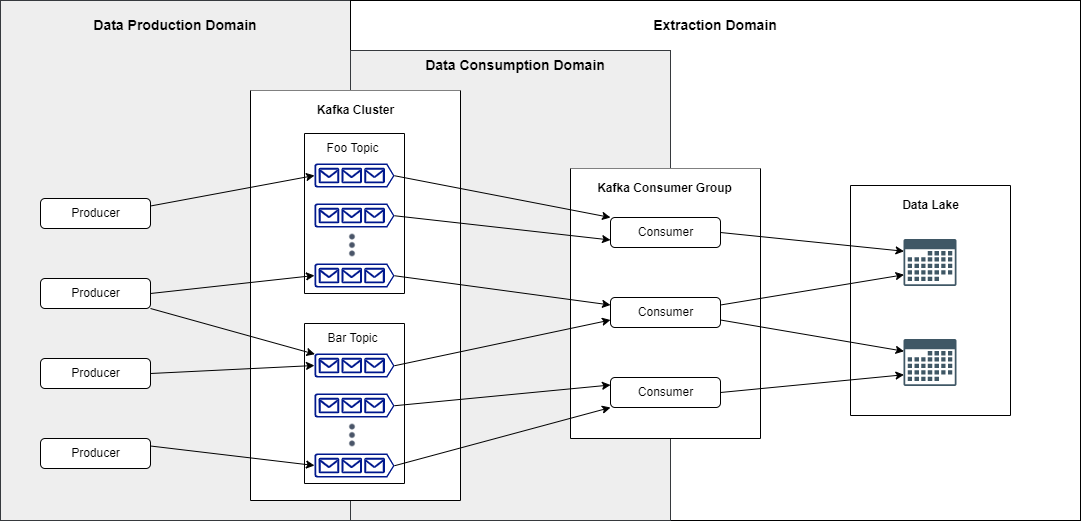
\includegraphics[width=\textwidth]{images/introduction/Context.png}
\caption{
    Data pipeline representing the flow of data since it is appended into one of
    the data sources (Topic), to when it is fetched by a consumer and inserted
    into a Data Lake.
}
\label{fig:problem_context}
\end{figure}

Throughout this work, we use Kafka as the message broker system. A Kafka cluster
is made of topics, which in turn is a unit that is subdivided into several logs,
commonly reffered to as partitions. When a producer sends a record to a specific
topic, it will be appended into one of the topic's partitions, illustrated in
the Data Production Domain in Figure \ref{fig:problem_context}. 

A consumer group is a unit composed of multiple consumers, each with the common
task of consuming data from the topics the group is subscribed to. To consume
the data within a topic, each of its partitions have to be assigned a single
consumer belonging to the same group. Assigning the partition's to different
consumers in a group, is Kafka's way of providing scalability. This design
feature leads to the fact that a group does not require more consumers than the
number of partitions, as only one consumer in a group can read data from a given
partition.

The problem was proposed by the data engineering team at HUUB (MAERSK), and it
is framed within the scope of the Extraction Domain in Figure
\ref{fig:problem_context}. It consists of being capable to dynamically manage a
group of consumers, to up- and down-scale the number of instances (i.e.
consumers), and also specify the tasks (partitions) that are assigned to each
consumer. We need to define the required amount of parallelism as to guarantee the
number of unread messages by the group does not increase with time. Hence, the
rate at which the group is consuming data from each partition, must be bigger or
equal to their respective write speed.

Considering consumers as bins, and partitions as items that have to be assigned
a bin, we model this problem as the Bin Packing Problem (BPP), with the
particularity that items vary in size with time. This occurs because the
partition's size correlates to its current write speed, which fluctuates based
on the current system's load and inevitably implies that a solution for a given
time instant may not hold true in future instants. 

On account of this BPP variation, a new solution has to be computed at each
instant, which might lead to a partition (item) being assigned to a different
consumer (bin) when compared to the consumer group's previous configuration.
Since two consumers cannot read from the same partition concurrently, the cost
associated to rebalancing a partition is related to the amount of data that is
not being read while the partition is being assigned to another consumer. 

Given that it is the first time the Bin Packing Problem is applied in this
context, existing algorithms do not take the rebalancing cost into account.
Hence, in Section \ref{sub:rscore} we propose a metric to account for a given
iteration's rebalance cost (Rscore). Additionally, using the Rscore, in Section
\ref{subsub:modified_any_fit} we propose four new BPP heuristic algorithms that
account for the rebalance costs.

The algorithms' performance is compared in section \ref{c3subsub:testing}. Since
the algorithms are attempting to solve a multi-objective problem that aims to
minimize both the number of bins required and the rebalance cost for a single
iteration, we compute the pareto front. It shows that three of the proposed
algorithms are a competitive solution to the problem at hand.

To deliver a fully automated solution to the autoscaling problem, in Chapter
\ref{chap:consumer_group_autoscaler} we introduce a system comprising three
components: a monitor, a consumer and a controller. Using the data from the
monitor process the controller uses the aforementioned theoretical approaches
(BBP heuristics) to assign tasks to consumers. Each of the components is
unitarily tested throughout Sections \ref{component:Monitor},
\ref{component:consumer} and \ref{component:controller}. An integration test is
also presented in Chapter \ref{chap:integration_tests}, aimed to reflect the
autoscaler's response time to the message broker's current load. Lastly, in
Chapter \ref{chap:conclusions}, we discuss results and suggest future work.
The following chapters introduce this thesis' technological and theoretical
background, Chapter \ref{chap:infrastructure} and Chapter \ref{chap:literature
review} respectively.


 
\chapter{Infrastructure} \label{chap:infrastructure}

\section{Distributed Systems Architecture}

When developing a digital infrastructure system, it is common to start with a
monolith approach where all application concerns are contained in a single
deployment, but it is hard to ignore its disadvantages as it can easily become
the bottleneck of the system. With monoliths, a lot more care has to be given to
how each part of the system communicates with one another, as communication is
achieved through method or function calls. This leads to very tight coupling
between different application components, which inevitably provides a lot of
friction to updating the codebase due to the high risk of it disabling the
service entirely.

Like with most applications, with every new feature the monolith grows, also
increasing the computing resources required to run a single instance. In times
of traffic peak, it is common for an application to scale its service allowing
for response speed to remain within acceptable times. The bigger the deployment,
the longer it takes to make a new instance available and the more computing
resources are used, making it more expensive to provide availability in times of
high traffic.

With this type of system, technological choices have a big impact on the final
product, and have to be thoroughly planned in the beginning to guarantee that
the system fulfills its requirements. It also makes it harder to adopt a
different technology further into the development due to the technological cost.
This point alone, makes it hard to accept this design, especially considering
the frequency of new advances in the field, and it is only natural that a new
approach to system architecture were developed.

Although there is no formal definition for what a microservice is,
\cite[Chapter~1]{newman2015building} states that ``Microservices are small,
autonomous services that work together.'' Small is of course a subjective
measure, but in fact there is no "theoretical" boundary on this quantity. It
depends on the context of the application and the business, but considering the
size of these microservices, it is only logical that each of the small services
follows some kind of team structure allowing for parallel development, without
any real coupling between the services. 

It is also stated in \cite{MartinFowlerMicroservices} that Microservices are
built around different ``business capabilities'' which are ``independently
deployable by fully automated deployment machinery''. In other words, each
microservice can be deployed on its own, hence scaling services and reliability
is "included" with this kind of architecture. This makes updating code very low
risk. As an example, in the scenario there is some flaw in a new deployment sent
to production, it will only affect that microservice in particular, making it
easier not only to track where the fault lies, but also guaranteeing that the
remaining services are not made fully unavailable.

On the topic of scaling, with smaller decoupled services, only the service that
requires scaling is in fact replicated, which leads to less computer resources
utilization thanks to the reduced overhead of the service, resulting in a
considerate cost reduction, and faster response to scaling needs.

With the possibility of running decoupled services interacting through
lightweight network calls, each microservice can be programmed in whichever
programming language and run the datastore that fits its needs best. The reduced
size of each service, also makes technological changes and code refactoring a
lot simpler, and can be done in a lot less time when compared to its counterpart.

It is also worth mentioning that the separation between each service allows
several representations of the same data in different ways depending on the
service that is storing it. The benefits of this approach is not only in a
projection perspective where there isn't a need to over-engineer how the data
will be stored for future purposes that still are not implemented, but it also
helps model the world in the way that fits each service best. 

Having multiple representations for the same data, also leads to inconsistency
in the data stored in the different services. Employing a data warehouse in this
scenario overcomes this hurdle, by unifying the data models of the different
services, and becoming the single source of truth for any representation of the
data within the system. It is also notably hard to maintain data consistency
between the distributed services, and on this note, the following section is
introduced.

\section{Distributed Messaging Systems}\label{sec:DMS}

When interacting between two distinct distributed servers, rarely should two
components communicate with one another directly or through synchronous
communication. If this were not the case, the communication would become too
convoluted with the increase of instances and services, becoming a source of
coupling. 

As stated in \cite{sharvari2019study}, it is clear the market needs point to a
messaging system that has the following features:
\begin{itemize}
    \item Scalable - the system provides tools with which services can process a
        bigger load of messages in a time of intense volume of traffic;
    \item Space decoupling – The receiving and sending entity do not need to
        “know” each other;
    \item Reliable – The system can guarantee that the receiver has received the
        message;
    \item Asynchronous  – The sender and receiver do not have to be active at
        the same time.
\end{itemize}

To enable decoupling between services, most messaging systems leverage the use
of a broker, providing with the space and time decoupling, with the added
benefit of it also being asynchronous, in the sense that after the broker
acknowledges the reception of the message sent by the producer, the producer
does not need to worry about its consumption allowing for it to go back to the
tasks it has at hand. There are two main approaches at solving this problem,
event and message driven paradigms.

\subsection{Message Driven}

This paradigm makes use of message queues where producers send the data for it
to be consumed by a single consumer in the same order it was appended to the
queue. When data is produced, in case there isn’t a consumer interacting with
the queue, the message is stored until read. 

RabbitMQ is a well known platform commonly used for this purpose. All the
previous features are provided, and on the note of scalability, a given service
can connect to a queue with one or more consumers to increase consumption rate.
This is done using round-robin dispatching \cite{RabbitMQscale} which simplifies
parallelizing work between instances, always guaranteeing that each message in a
queue will be read by a single consumer.

\subsection{Event Driven (Publish/Subscribe)}

Messaging system which allow a producer to send a message to a certain category,
which can be posteriorly retrieved by multiple consumers which are subscribed to
the same category. This architecture not only decouples the services, it also
allows many-to-many communication.

A common application for the event driven paradigm is for event sourcing. This
is the pattern of storing any event that changes a system's state via an event
object, onto an event log that preserves the sequence in which the events
occurred. This is presented as an alternative to storing structures that model
the state of the world, into storing events that lead to the current state of
the world \cite[Chapter~5]{nadareishvili2016microservice}.

Comparing this scenario to the one of using a database, in the latter, every
time the main database is updated, a second database recording the historic
state has to be updated as well, storing the past states the system has been
through. With event sourcing, when an event changes the state of the system, it
is simply appended to the sequential event log, which in turn makes it less
expensive to make operations of this type.

\section{Kafka}

Kafka functions as a distributed log running in multiple brokers that coordinate
with each other to form a cluster.

\begin{figure}[H] 
    \centering
    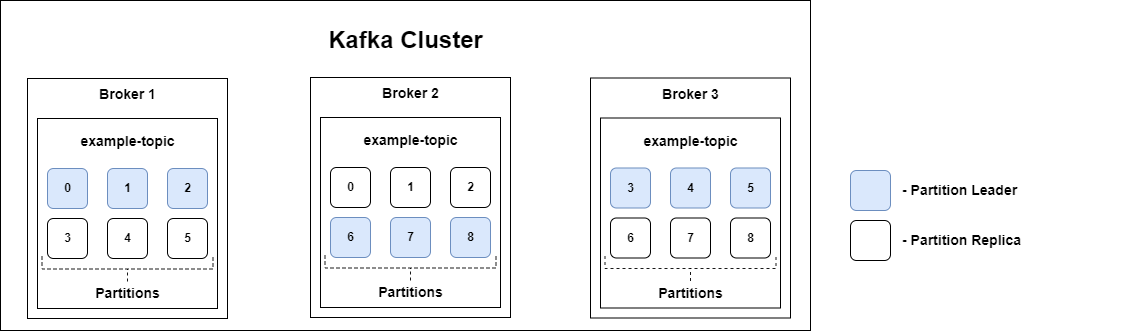
\includegraphics[width=\textwidth]{images/infrastructure/Kafka Cluster.png}
    \caption{
        Representation of a Kafka Cluster composed of three brokers, with a
        single topic (Example Topic), containing 9 partitions and a
        replication factor of 2.
    } 
    \label{fig:kafka_cluster} 
\end{figure}

\subsection{Broker}

A Kafka cluster is made up of one or more brokers, which function as servers
where the messages can be published to, and consumed from. This is the entity
each client has to connect to in order to interact with Kafka. After a client
connects to a single broker, it will also be connected to the remaining elements
of the cluster.

\subsubsection{Topics and Partitions}

When data is published, the producer has to specify to which topic the record
goes to. A topic contains several partitions, and each partition can be stored
in different brokers. Message order is only guaranteed within a single
partition.

At the time of topic creation, there are three parameters that have to be
provided: 
\begin{enumerate}
    \item \textbf{topic} - The name of the topic to create;
    \item \textbf{partitions} - The amount of partitions the topic is subdivided
        in;
    \item \textbf{replication-factor} - The amount of replicas of each partition
        to guarantee a reliable service.
\end{enumerate}
The \lstinline{example-topic} presented in figure \ref{fig:kafka_cluster} would have been
configured with \lstinline{topic=example-topic}, \lstinline{partitions=9} and
\lstinline{replication-factor=2}.

Although the first two parameters are self-explanatory, the third is one of the
most important features to guarantee a reliable service to a producer. 

Assuming the scenario of choosing the replication factor of 2, this means that
for each partition in the created topic, there will be 2 partitions that
represent the same log in different brokers. At any given time, there is only 1
partition leader (broker), which leaves the other partition trying to keep up
with the main log. When a replica is up-to-date with the leader, it becomes an
in-sync replica (ISR). If a partition leader fails unexpectedly, the partitions it is
leading have to be reassigned a different leader. For each partition, the new
partition leader will be one of the brokers that contains an in-sync replica of
the same partition.

\subsection{Producer}

To publish data, producers have to connect to one of the brokers from the
cluster, which will automatically inform the client as to how to connect to the
remaining brokers of the same cluster. When sending a record, the producer
has to specify the topic to which the record is to be added, and may optionally
provide other parameters which will impact the partition the record will be
added to. If no additional parameter is provided, a random partition is selected
to which the record is added.

\begin{figure}[hbt!] 
    \centering
    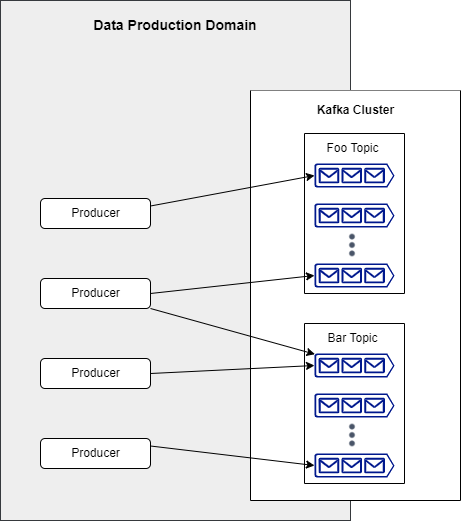
\includegraphics[width=0.5\textwidth]{images/infrastructure/Production Domain.png}
    \caption{
        Data production representation within the Kafka Ecosystem.
    } 
    \label{fig:data_production_domain} 
\end{figure}

For a single partition, the log that belongs to the partition leader (shaded
partitions in figure \ref{fig:kafka_cluster}) is where the messages are appended
to and read from. To guarantee a message is delivered safely to the cluster, a
producer might want to wait for acknowledgement. This is one of the
configurations that allows for reliability when adding a message to a topic
\cite{KafkaProducer}. In figure \ref{fig:data_production_domain}, the partitions
presented are only the leader partitions within the topic.

There are 3 possible values for this configuration:
\begin{itemize}
    \item \lstinline{acks=0} - Producer does not wait for acknowledgement, making it an
        unreliable configuration;
    \item \lstinline{acks=1} - Producer waits for acknowledgement from the partition
        leader;
    \item \lstinline{acks=all} - Producer expects an acknowledgement from leader and all
        of its replicas.
\end{itemize}

After appending data to a log, it can no longer be changed (immutability).
Additionally, when producing a message, if the order of a group of messages is
important, Kafka provides a feature that allows messages to be consumed in the
same order as they were produced. This is done by setting the key of a record to
the same value, having a hash function run over the key, and the partition where
the message goes to is consistently the same, while the number of partitions in
the topic does not change. If the number of partitions changes, this is no
longer the case.

\subsection{Consumer Group and Consumer Clients}
\label{sec:kafka_consumer_group}

When connecting a consuming client to the messaging system, the topic(s) it
wishes to subscribe to, the consumer group id and at least one of the brokers from
the cluster have to be provided (a connection to a single broker connects the
consumer to all the other brokers in the cluster). 

\begin{figure}[hbt!] 
    \centering
    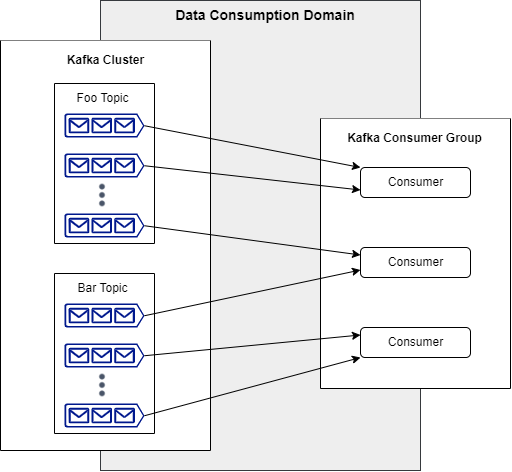
\includegraphics[width=0.6\textwidth]{images/infrastructure/Consumption Domain.png}
    \caption{
        Representation of the consumption process for a Kafka Consumer Group.
    } 
    \label{fig:data_consumption_domain} 
\end{figure}

Messages are then read in order w.r.t a single partition, and in parallel w.r.t.
multiple partitions. Each consumer from within a consumer group, reads from
exclusive partitions.  This means that two consumers belonging to the same
consumer group cannot be responsible for reading messages from the same
partition, which in turn implies that the parallelism Kafka provides, is through
the partitions in a topic. The amount of active consumers a single consumer
group can have is therefore limited to the total amount of partitions in the
topics the consumer group is subscribed to \cite{OreillyConsumer}. 

In order to maintain a reliable consumption service, whenever a consumer
successfully reads a message and commits its offset, kafka internally stores the
offset in a topic with the name \lstinline{__consumer_offset}
\cite{KafkaConsumer}. This internal topic has another functionality which is
related to the consumer group management. For a group to know when to rebalance
it is important for the system to monitor the state of each consumer in the
group, and this is performed by a group coordinator. To elect a group
coordinator, the consumer group's id is selected as the message key, which is
then hashed into a partition of this internal topic. The broker which is
partition leader of this partition becomes the group coordinator.

For a consumer to remain a member of the group, it must periodically send
heartbeats with a predefined interval to the coordinator. When the maximum
amount of time without receiving a heartbeat is exceeded or the coordinator is
notified of a consumer leaving the group, rebalancing is triggered, reassigning
the partitions the consumer was responsible for to the remaining elements of its
group.

The same rebalancing is triggered when a consumer starts up and requests to join
a group. Rebalancing is simply attempting to split the load between the active
consumers of a group, and Kafka's group coordinator does this by assigning
approximately an equal amount of partitions to each consumer in a group. 

Depending on the chosen configuration for the parameter
\lstinline{auto.offset.reset}, when a consumer receives its assignment from the
coordinator, if there are no committed offsets by the consumer group's id for
the topic-partition pair, then this policy is selected to determine where to
start consuming records from its partitions. If it is set to \lstinline{earliest}
it will start consuming from the first message in the partition, whereas if set to
\lstinline{latest} it will start consuming from the last message appended to that
partition's log.

When data is consumed in batch, it can only be guaranteed that the data is read
at least once. The reason why this is the case is due to the fact that if a
consumer fails while processing the messages, before committing the offsets, the
partition is reassigned and the same messages will be read again. To define the
size of the batch, a combination of the following parameters,
\lstinline{max.partiiton.fetch.bytes} and \lstinline{fetch.max.bytes}, provides
more granular control. If the number of duplicate messages is relevant, the
batch size is an important factor to take into consideration, since the bigger
the size, the more messages can be read more than once in cases of consumer
failure.

While rebalancing, it is important to note that the consumers are not capable of
consuming data from the partitions being rebalanced, making it an expensive
operation which is to be avoided. If a certain consumer stops unexpectedly, it
is no longer consuming from its partitions, and the coordinator has to wait for
as long as \lstinline{session.timeout.ms} for it to trigger a rebalance. This is a
configurable value, but there is of course a trade-off. The bigger the value
set, the less rebalancing is performed, but it will also take the coordinator
longer to determine whether a single consumer is unavailable before triggering a
rebalance. 

\section{Containers} \label{sec:COM}

When internet services first started, it was common to have the services running
on local hardware. To handle peak traffic, scaling was performed by purchasing
more hardware, which would then become unused when the traffic was no longer as
high \cite[Chapter~1]{smith2017docker}.

Virtual Machines (VMs) became the next advance in this industry, and it allowed
to use the resources of pieces of hardware more efficiently as multiple VMs
could run on a single machine as long as there was space. This is when cloud
service providers like Amazon, Google and Microsoft also started renting out
VMs. In moments of peak traffic, a company could scale services in minutes, and
there was no need to waste hardware resources with unused instances, therefore
paying only for what is used.

It became clear that Virtual Machines also came with disadvantages, as there was
a considerable overhead of memory to support the operating system of this
environment.

Enter containers. Running instances could be done in a matter of seconds without
the overhead of an operating system, which allows applications to run
consistently in different environments as long as the containers are created
resorting to the same image.

As stated in \cite{DockerContainer}, an image is a bundle of code/software which
contains all the dependencies and libraries a given instance might need to run
reliably in different computing environments. Container images become containers
on runtime.

\section{Kubernetes} \label{subsec:kubernetes}

Kubernetes works with a cluster of distributed nodes, that interact with one
another to work as a single unit. This service allows for an automated
distribution and scheduling of containerized applications. The level of
abstraction causes a deployment to have no ties to a specific machine.

A kubernetes cluster is formed by 2 entities, the control plane, and nodes. The
first is responsible for coordinating all activities in a cluster, such as
scheduling, scaling and rolling out new updates of an application. The second,
contains a process named kubelet, which manages the communication of the node
with the control plane. There are additional tools like containerd or docker to
allow the node to deploy containerized applications.``In practice, a node is
simply a VM or a physical computer that serves as a worker machine in
Kubernetes'' \cite{CreateKubeCluster}.

As soon as the Kubernetes cluster is running, it is possible to deploy the
containerized applications. This can be done using one of the many resource
types, such as a \textbf{Deployment}. It is within this type of resource that we can
specify how our applications will run, and how many instances of the application
we want to make available. Within the deployments \lstinline{spec.replicas} is
where we define the number of pods we want the deployment to contain, and within
\lstinline{spec.template} is where the Pod resource is specified for this
deployment. A \textbf{Pod} is Kubernetes smallest deployable resource, and it is an instance
that runs within a single Node. It can run one or more containers that are
created using their respective images, which share network and volume resources.

When up- or down-scaling the deployment, \lstinline{spec.template} is always
used to determine the Pod instance to manage.  Within the deployment's spec
field, which specifies the resource's state,
\lstinline{spec.selector.matchLabels} and
\lstinline{spec.template.metadata.labels} are what allows a deployment to know
which pods to manage. The pods are tagged with the label specified by
\lstinline{spec.template.metadata.labels} and the deployment searches for the
pods have the labels specified in \lstinline{spec.selector.matchLabels}. 
At all times, there is a deployment controller that continuously monitors the
instances. 

In the scenario the node running a given instance fails, the
controller detects the failure and launches the same instance on another node
that belongs to the cluster. This is a consequence of the control plane
attempting to maintain the state of an application that was defined in the
deployment configuration.

Kubernetes offers a command line interface (CLI), kubectl, which gives a user the possibility to
communicate with the cluster locally. The communication is performed via the
Kubernetes API, which is an API server located on the control plane. This server
exposes an HTTP API, which allows differing entities to interact with it to
query or even change API object's states \cite{KubernetesAPI}. 

A clusters API server is the core of the control plane. This HTTP API, allows
differing entities to communicate with the cluster and manage kubernetes
objects. To manage a consumer group, the controller described in section
\ref{component:controller} leverages this API to create deployment and volume
resources.

\subsection{Autoscaling}

As described in \cite{KubernetesAutoscaling}, the algorithm works in loop,
constantly evaluating the performance of the pods measuring the average CPU
usage in the last minute. The control is performed by default every 30s, which
can be modified by changing the value of
\lstinline{horizontal-pod-autoscaler-sync-period}.

The following equation determines the appropriate amount of pods, so as to have
the average $CPUUtilization$ for the pods within a deployment below the target:
\begin{equation}
    numPods = ceil\bigg(\frac
        {\sum_{p \in Deployment} CPUUtilization_p}
        {Target}
    \bigg)
\end{equation}
where $CPUUtilization_p$ is the average CPU utilization in the last minute of a
pod $p$. 

To reduce noise in the metrics, the autoscaler can only scale-up if there was no
rescaling within the last 3 minutes. The same applies to scale-down but the
waiting time is 5 minutes.

Within the context of the problem presented in section \ref{chap:intro}, if a
pod represents a consumer and a deployment a consumer group, the metric on
which to base the autoscaling cannot be the deployment's average CPU
utilization, as the process shown in figure \ref{fig:problem_context} utilizes
more network than processing resources. 

Kubernetes Event Driven Autoscaling (KEDA), provides a Kafka Consumer Group
scaler which allows to increase the amount of consumers based on the average lag
of a consumer group. Although this is definitely better than scaling based on
the CPU usage, it still lacks granularity on evaluating the groups performance
based on other metrics, providing as an example, consumption and production rate
of a partition. The load is also distributed between the consumer instances
using the strategy mentioned in section \ref{sec:kafka_consumer_group}, where
the aim is to assign approximately the same amount of partitions to each
consumer within a group. Since the speed of each partition to be assigned is not
the same, this is does not equally split the load between the consumers.

\subsection{Kubernetes Operating Modes}

When running Kubernetes, there are several alternatives. The first is to have
the cluster run on manually provisioned hardware, which provides with the most
control over which type of node is added or removed from the cluster. 

As soon as a node is manually added to the cluster, the control plane can start
assigning pods to run in the node. When there is no longer any more space in the
cluster to run other instances, more nodes have to be added to the cluster to
allow the deployments to be correctly scheduled to maintain the state described
in the deployment.

With this type of configuration, the operational cost is usually associated with
the nodes that are added to the cluster, which can represent renting out VMs or
buying the actual physical hardware that runs the necessary software to be a part
of the Kubernetes cluster.

Another option is to use some kind of cluster auto-management which is
already included in a few cloud provider's Kubernetes Engine. Using as an
example Google's Kubernetes Engine (GKE), there is a cluster mode of operation
(autopilot), that manages the nodes within the cluster automatically
without having to manually interact with the cluster. This means that if the
cluster does not have enough resources to maintain the state of the objects that
are within the cluster, a node is automatically added, and the
instances that require node resources can now be scheduled.

This mode of operation allows the user to pay by pod instead of node
\cite{GKEautopilot}, meaning that only the resources that are being used are
being payed for. Autopilot allows a truly dynamic and hands-off experience when
dynamically scaling a certain deployment.

\chapter{Bin Packing Problem} \label{chap:literature review}

The bin packing problem (BPP), as defined in the literature, is a combinatorial
optimization problem that has been extensively studied since the thirties. As
specified in \cite{wascher2007improved}, there are several categories with which
to define a BPP. The problem at hand is the one of a Single Bin Size Bin Packing
Problem (SBSBPP). As described in \cite{delorme2016bin}, an informal definition
of this BPP, is: provided there are n items, each with a given weight \( w_j  \,
(j = 1, ..., n) \) and an unlimited amount of bins with equal capacity \( C \),
the goal is to arrange the n items in such a way that the capacity of each bin
is not exceeded, and to determine the minimum amount of bins required to hold
the $n$ items.

Formally, the problem can be summarized as the following optimization problem:
\begin{alignat}{3}
    &\min       
        &&\sum_{i \in B} y_i 
            && \\
    &\text{subject to} \quad
        && \sum_{j \in L} w_j \cdot x_{ij} \leq C \cdot y_i \quad      
            && \forall \; i \in B \label{opt:c1} \\
    &   && \sum_{i \in B} x_{ij} = 1, \quad                 
            && \forall \; j \in L \label{opt:c2} \\
    &   && y_i \in \{0, 1\}                                 
            && \forall \; i \in B \\
    &   && x_{ij} \in \{0,1\}                               
            && \forall \; i \in B, j \in L
\end{alignat}
where set $B$ corresponds to the available bins, and $L$ as the list of items to
be arranged into different bins. $x_{ij}$ indicates whether an item $j$ is
packed in the bin $i$, whereas $y_i$ informs whether bin $i$ is used. 

As for the constraints, \ref{opt:c1} assures that the sum of the items in a bin,
does not exceed it's capacity, and \ref{opt:c2} makes sure that every item is
assigned a bin. 

It is also common to represent the bin-packing problem in its normalized
version, where all the weights are down-scaled by the total capacity of a bin,
and the capacity of each bin is $1$. This implies modifying \ref{opt:c1} into:

\begin{equation}
    \sum_{j \in L} \hat w_j \cdot x_{ij} \leq y_i \quad \forall \; i \in B,
\end{equation}
where \(\hat w_j\) represents the normalized weight of an item ($w_j/C$).
Throughout the following anaylsis, both "weight" and "size" will be used
interchangeably, and the normalized BPP model will be employed.

\section{Linear Programming}

When interested in achieving the optimal solution, the textbook implementation
of the BPP model presented by equation \ref{BPP model} is not computationally
efficient. A common approach is to study the Upper and Lower Bounds of the
Algorithm, and to add valid additional constraints to restrict the search space.

In \cite{delorme2016bin}, there is an extensive review on the state of the art
algorithms that have been developed to solve the ILP problem, comparing several
models and their efficiency when solving the same set of problems. 

Wihtin the context of the problem presented in chapter 1, provided two time
instants $t_1$ (the last instant at which the item assignment was computed) and
$t_2$ (the current time instant at which the assignment is to be re-computed),
given that the items' sizes change between $t_1$ and $t_2$, it is possible that
the configuration computed in $t_1$ no longer complies with constraint
\ref{opt:c1}. Considering the NP-hard nature of the problem, and the fact that the
ILP problem is only interested in minimizing the amount of bins disregarding an
item's previous assignment, this thesis will give more emphasis to the
Approximation Algorithms that provide more control over the item reassignment
problem, and provide a solution within the strict time constraints imposed by
the real-time requirements presented in chapter \ref{chap:intro}.

\section{Approximation Algorithms and Heuristics}
\label{section:AA}

In \cite{coffman2013bin} a method is presented to classify the BPP problem,
which will be used throughout this section. During an algorithm's execution,
a bin can find itself either \textit{open} or \textit{closed}. In the former,
the bin can still be used to add additional items, whereas in the latter, it is
no longer available and has already been used.  

In the literature, it is common to present a parameter $\alpha$ which
indicates the size limit of the weights within the list $L$, which varies
between $(0, 1]$. This thesis studies the problem where the item's size is
simply limited to the size of the bin, and therefore $\alpha = 1$.

To compare the performance between algorithms, the Asymptotic Performance Ratio
(APR), is what will be employed throughout this section. $A(L)$ denotes the
amount of bins a certain algorithm makes use of for a configuration of items
$L$. $OPT(L)$ is used to represent the amount of bins required to achieve the
optimal solution. Defining $\Omega$ as the set of all possible lists, each with
a different arrangement of their items, given
\begin{equation}
    R_A (k) = \sup_{L \in \Omega} \left \{ \frac{A(L)}{k} : k = OPT(L) \right \},
\end{equation}
the APR is defined as
\begin{equation}
    R_A^\infty = \limsup_{k \to \infty} R_A(k).
\end{equation}

Despite the mulititude of classes presented in \cite{coffman2013bin}, the only
classes of problems that are of interest for this thesis are: 
\begin{enumerate}
    \item online - Algorithms that have no holistic view over any other item in
        the list except the one it is currently assigning a bin to. It is also a
        requirement that an item is assigned a bin as soon as it is analyzed.
    \item bounded-space - The amount of bins open at a single instance is
        limited by a constant provided prior to its execution.
    \item offline - The algorithm is aware of all the items in the list before
        assigning bins to each item, and so their ordering does not directly
        impact the outcome as it is not necessary to respect the list's initial
        order.
\end{enumerate}

\subsection{Online Algorithms}

Whenever an item is analyzed it has to be assigned a bin. This also implies that
the bin in which the current item will be inserted is a function of the weights
of all the preceding items in the list.

This section will analyze Any fit, Almost any fit, bounded-space and reservation
technique algorithms.  Throughout the following sections, when \textit{current
item} is mentioned, it is referring to the next item to assign a bin to. After
assignment, the item that follows it in the list, is then considered the
\textit{current item}.

\textbf{Next Fit (NF)} is one of the simplest algorithms developed to solve the
bin packing problem heuristically, and it consists in the following procedure.
The current bin is considered to be the last non-empty bin opened. If the
current bin has space for the item then the item is inserted. Otherwise, the
current bin is closed, a new one is opened, and the item is inserted. The next
item on the list is then considered the current item.

With regards to time complexity, NF is $O(n)$. And because there is only one
open bin at a time, this is a bounded-space algorithm with $k = 1$. As proven in
\cite{johnson1973near}, 
\begin{equation}
    R_{NF}^\infty = 2.
\end{equation}

\textbf{Worst Fit (WF)}: For each element, it looks for the open bin that has
the most space where it fits, and inserts the item in that bin. If there is no
open bin that can hold the item, then a new bin is opened, and the item is
inserted. Having no closing procedure, this algorithm is unbounded, and it does
not run in linear time.

Although it is expected that this algorithm would perform better than the NF, in
the worst-case performance analysis it does not gain any benefits from not
closing its bins, as stated in \cite{man1996approximation}
\begin{equation}
    R_{WF}^\infty = R_{NF}^\infty.
\end{equation}

\textbf{First Fit (FF)} searches each open bin starting from the lowest index,
and the first bin that has the capacity to fit the item, is where the item is
inserted. If there is no open bin where the item can be inserted, then a new bin
is opened where the item is inserted. In \cite{johnson1974worst} it is shown
that
\begin{equation}
    R_{FF}^\infty = \frac{17}{10}.
\end{equation}

There is a more general class of algorithms presented as \textit{Any Fit} ($AF$)
in \cite{johnson1974fast}. This class' constraint is that if $BIN_j$ is empty,
then no item will be inserted into this bin if there is any bin to the left of
$BIN_j$ that has the capacity to contain the item. In the same paper it is also
shown that no algorithm that fits this constraint can perform worst than the WF,
nor can it perform better than the FF, always with respect to the asymptotic
performance ratio. Then
\begin{equation}
    R_{FF}^\infty \leq R_A^\infty \leq R_{WF}^\infty, \; \forall \; A \in AF
\end{equation}

\textbf{Best fit (BF)}: Attempts to fit the item into any of the open bins where
it fits the tightest. If it doesn't fit in any, then a new bin is created and
assigned to the item. As can be seen, it is similar to the worst fit, with
exception to the fitting condition, differing only in the fact that the item is
inserted where it fits the tightest, and not where it leaves most slack.

As it happens, BF also belongs to the $AF$ class, and it performs as well as the
First Fit
\begin{equation}
    R_{BF}^\infty = R_{FF}^\infty.
\end{equation}

In \cite{johnson1974fast}, a another class of algorithms presented, which is
also a subclass of $AF$, is \textit{Almost Any Fit} ($AAF$). This class has as
constraints: \textit{If $BIN_j$ is the first empty bin, and $BIN_k$ is the bin
that has the most slack, where $k < j$, then the current item is not inserted
into $k$ if it fits into any bin to the left of k.} One of the properties proven
in the same paper, is that 
\begin{equation}
    R_A^\infty = R_{FF}^\infty, \; \forall \; A \in AAF,
\end{equation}
which is to say that any algorithm that fits the previous constraints, have the
same APR as the FF algorithm. Focusing on the constraints, it is clear to see
how BF and FF belong to this class. 

Due to the constraints presented in the $AAF$ class, an improvement for the WF
algorithm arises wherein the current item is inserted in the second bin with
most space, instead of the first. This algorithm is the Almost Worst Fit (AWF),
and with this simple change, now belongs to the AAF class, having as APR
\begin{equation}
    R_{AWF}^\infty = R_{FF}^\infty = \frac{17}{10}.
\end{equation}

\subsection{Bounded-space} 

Bounded-space algorithms have a predefined limit on the amount of bins that are
allowed to be open at a given instance, which will be defined as $k$. It is also
a subclass of the online algorithms.

An example of a bounded-space algorithm is NF, as it never has more than a
single open bin at a given instant. The other presented online algorithms can
also be adapted into a bounded space algorithm, simply by specifying a procedure
as to which bin to close before exceeding the limit.

A bounded-space algorithm can be defined via their packing and closing rules
\cite{coffman2013bin}. A class that derives from rules based on the FF and BF
can be defined in the following manner: 
\begin{itemize}
    \item Packing - When packing an item into one of the available open bins,
        the selected bin either follows a FF or BF approach.
    \item Closing - When choosing which bin to close, if following the FF
        approach, then the bin with the lowest index is closed. If following the
        BF it's the bin that is filled the most that is selected as the one to
        be closed.
\end{itemize}

The notation for this class of algorithms is $AXY_k$, where X represents the
packing rule, and assumes the letters $F$ or $B$, and $Y$ which can either be an
$F$ or a $B$, refers to the closing rule. The $k$ represents the maximum amount
of open bins allowed.

\textbf{Next-k-fit} applies both packing and closing rules based on the first
fit algorithm, and as expected when $k \to \infty$ it approximates the FF
algorithm, having as APR $17/10$. As shown in \cite{mao1993tight}

\begin{equation}
    R_{AFF_k}^\infty = \frac{17}{10} + \frac{3}{10k - 10}, \quad \forall \; k \geq 2.
\end{equation}

\textbf{Best-k-fit}, which is also known as the $ABF_k$ algorithm, has been
proven in \cite{mao1993besk} to have
\begin{equation}
    R_{ABF_k}^\infty = \frac{17}{10} + \frac{3}{10k}, \quad  \forall \; k \geq 2.
\end{equation}

As for $AFB_k$, \cite{zhang1994tight} showed that this algorithm has
\begin{equation}
    R_{AFB_k}^\infty = R_{AFF_k}^\infty, \quad  \forall \; k \geq 2.
\end{equation}

For the last possible combination of this class of algorithms, $ABB_k$ has been
proven in \cite{csirik2001bounded} to have 
\begin{equation}
    R_{ABB_k}^\infty = \frac{17}{10},  \quad \forall \; k \geq 2
\end{equation}
which surprisingly indicates that the value of $k$ (as long as it's bigger than
two) has no effect on the APR metric of this algorithm, contrary to all the
previous algorithms.

The next algorithms make use of a reservation technique that proved to be very
useful to break the lower bound of the APR of the Any Fit class of algorithms.
The first algorithm to be developed of this type was the Harmonic-Fit ($HF_k$)
which makes use of k to split the sizes of items into $k$ different intervals.

$I_j$ denotes the interval of sizes with index j, and is within the range 
\begin{equation}
    \left (\frac{1}{j+1}, \frac{1}{j} \right], \quad \forall \; j \in \{1, ..., k-1\}.
\end{equation}
$I_k$ is defined as the interval from $(0, 1/k]$.

$B_j$ is used to classify the bin type which is responsible for holding items of
type $I_j$.

It is shown in \cite{lee1985simple} that for $HF_k \forall k \geq 7$ the
algorithm already performs better than the other online bin packing algorithms
presented, with regards to the APR.

Posterior to this technique being presented, it was clear that the reservation
technique could be a good approach to improve the performance of the Any-Fit
algorithms, and as such, several other algorithms have been created around this
technique, that achieve even better APR's than HF, but because these techniques
all involve assigning item types, based on their size, to their respective bin
type, this approach is not applicable to the problem, as the control over item
rebalancing is reduced, which will further be described in the following
chapter.

\subsection{Offline Algorithms}

Comparing with the previous section, offline algorithms have the added benefit
that all items are known prior to its execution. As long as the set of items
remains the same, items can be grouped, sorted or anything that might be
convenient for the algorithm that is going to execute over the list of items. 

It is important to note that as soon as an algorithm chooses to sort the list of
items, it automatically implies that the algorithm no longer runs in linear-time
as the sorting algorithm would have a time complexity of $O(n log(n))$.

Most of the Any Fit algorithms, perform best if the list of items is sorted in a
non-increasing order. The following three algorithms remain the same as for how
the packing is done when analyzing the list of items, with the exception that
before running the algorithm, the list is sorted.

Provided the list is sorted in the aforementioned manner, the \textbf{Next Fit
Decreasing (NFD)} has a considerable improvement in terms of it's worst-case
performance, and performs slightly better than FF and BF, as presented by
\cite{baker1981tight}
\begin{equation}
    R_{NFD}^\infty \approx 1.6910.
\end{equation}

As can be seen in \cite{johnson1974worst}, \textbf{Best Fit Decreasing (BFD)}
and \textbf{First Fit Decreasing (FFD)} improve the APR metric with presorting
compared to their online versions of the same algorithm 
\begin{equation}
    R_{BFD}^\infty = R_{FFD}^\infty = \frac{11}{9}.
\end{equation}

Another algorithm which is worth mentioning within this class of offline
algorithms is the \textbf{Modified First Fit Decreasing (MFFD)}. As shown in
\cite{johnson19857160}, The APR is
\begin{equation}
    R_{MFFD}^\infty = \frac{71}{60},
\end{equation}
which is achieved by initially presorting the items in a decreasing manner and
grouping each item into seven distinct groups based on the item's size. 

\begin{table}[H]
\caption{Item size interval which guides the grouping for the MFFD algorithm.}
\begin{center}
\begin{tabular}{ |c|c| } 
    \hline
    Group & Item size interval \\ 
    \hline
    A & $\left( 1/2, 1 \right]$ \\ 
    B & $\left( 1/3, 1/2 \right]$ \\ 
    C & $\left( 1/4, 1/3 \right]$ \\ 
    D & $\left( 1/5, 1/4 \right]$ \\ 
    E & $\left( 1/6, 1/5 \right]$ \\ 
    F & $\left( 11/71, 1/6 \right]$ \\ 
    G & $\left( 0, 11/71 \right]$ \\ 
\hline
\end{tabular}
\end{center}
\end{table}

After doing so, the algorithm then performs the following five steps: 
\begin{enumerate}
    \item For each item that belongs to group A, from biggest to smallest,
        assign it a bin with the same index as the item has within it's group.
        When this process terminates, there are as many bins as items in group A
        and the bins created are $B_1, ..., B_{|A|}$.
    \item Iterating over the existing bins from left to right, for each bin, if
        any item in group $B$ fits in the bin, insert the biggest such item in
        the current bin.
    \item Iterating through the list of bins from right to left, for each bin,
        if the current bin contains an item that belongs to group $B$, do
        nothing. If the two smallest items in $C \cup D \cup E$ do not fit, do
        nothing. Otherwise insert the smallest unpacked items from $C \cup D
        \cup E$ combined with the largest item from $C \cup D \cup E$ that will
        fit.
    \item iterate over the list of bins from left to right, and for each bin if
        any unpacked item fits, insert the largest such item, repeating until no
        unpacked item fits.
    \item Lastly, the remaining items that did not fit in bins $B_1, ...,
        B_{|A|}$ are inserted in an FFD fashion starting with a new bin
        $B_{|A|+1}$. 
\end{enumerate}

\section{Bin Packing Applications}

There are several applications where the BPP is used to provide with an optimal or
sub-optimal solution. In \cite{baldi2019generalized}, the problem is modeled as
a BPP to solve the last mile delivery problem a courier usually faces when
having to decide which transportation companies are to be used to deliver the
parcels to the customers. In this case, a Transportation Company (TC) represents
a type of bin, and a vehicle of a TC represents a bin instance. The problem is
formulated as a generalization of the BPP, considering a profit value is
incorporated into the cost function which is based on the bin-type each item
ends up assigned to, which in the problem's context, this profit represents the TC's
QoS. As such, the objective function aims to minimize the net cost related to
the vehicle instances used to allocate the parcels and the profits associated
with the parcel assignment.

Another application where the BPP proves itself useful is in the The Virtual
Machine Placement (VMP) problem, which has gained more attention due to
increasing use of cloud providers to support companies' technological
infrastructure. Usually the problem can be generalized to a set of tasks
(Virtual Machines), each having to be assigned one of the cloud provider's
physical machines while attempting to minimize the operational cost. A variation
of the BPP is usually presented in this case where the items are considered
ephemeral and add another temporal dimension since they have associated a start
time and a duration during which the task has to be ran uninterrupted. 

In \cite{de2016temporal} the tasks have an equal start time and the aim is to
minimize the unused capacity of a physical machine over time, and therefore the
optimal solution for the BPP does not necessarily provide the optimal solution
in their Temporal Variant of the BPP (TBPP). In addition to the temporal model
presented by \cite{de2016temporal}, in \cite{aydin2020multi} the tasks may have
differing start times, and the objective function presented is more in line with
the traditional BPP where the number of physical machines required is minimized.
Moreover, due to the increased energy costs related to machine fire-ups
(switching a machine off when it is not in use and back on again when required),
the authors also attempt to minimize the number of fire-ups, making their
problem multi-objective.

As presented in \cite{furini2018matheuristics}, provided a set of items $N =
\{1,2,...,n\}$, a weight $w_i \; \forall i \in N$, and a start and end time
$[s_i, t_i[$, the set of items which have to be executing at a time instant
$s_j$ is $S_j = \{n \in N: s_n \leq s_j \; and \; t_n > s_j\}$. This allows the
definition of the non-dominated set $T = \{n \in N: S_k \subseteq S_n\}$ which
discretizes the time dimension into several time instants. Due to the stateful
nature of the problem that allows a task to be in more than one $S_j$, which
implies an item may have an assignment from a previous time instant, and since
an item cannot be rebalanced, an optimal solution for the $BPP(t)$ is not the
same as an optimal solution for $TBPP(t)$.

\section{Conclusion}

Although the temporal aspect of the Bin Packing Problem has already been
reviewed, there is a gap when it comes to the possibility of rebalancing the
items between the different bin instances, which is one of the aspects this
thesis aims to cover. 

This provides the basis for the work that will be developed. The objective is to
compute different instances of the BPP over time to guarantee that a consumer
group does not fall behind on the messages sent to the partitions that the group
is reading data from. 

% \section{Distributed Consumer Performance}

% \section{Filters}

%\section{Summary}

\chapter{Consumer Group Autoscaler} \label{chap:consumer_group_autoscaler}

Due to the dynamic nature of the problem presented in chapter \ref{chap:intro},
the items change in size depending on the measurement performed at time instant
$t$. Consequently, constraint \ref{opt:c1} is remodeled to take the time instant
$t$ at which the algorithm is to be executed into account.
\begin{alignat}{3}
\label{BPP model}
    &\min       
        &&\sum_{i \in B} y_i 
            && \\
    &\text{subject to} \quad
        && \sum_{j \in L} \hat w_j(t) \cdot x_{ij} \leq y_i. \quad      
            && \forall \; i \in B \\
    &   && \sum_{i \in B} x_{ij} = 1, \quad                             
            && \forall \; j \in L \\
    &   && y_i \in \{0, 1\}                                             
            && \forall \; i \in B \\
    &   && x_{ij} \in \{0,1\}                                           
            && \forall \; i \in B, j \in L
\end{alignat}

Time instant $t$ represents an instant at which a measurement was performed
of the items' sizes, leading to a new computation of the bin packing assignment.
Since an assignment represents a consumer reading data from the partition, an
item can also be reassigned to another consumer (bin) adding a new variation to the
traditional BPP. 

The Data-Engineering (DE) team at HUUB is responsible for making a pipeline that
inserts data from several data sources into a data lake so it can then be
transformed and loaded into a single source of truth data warehouse. 

HUUB's current architecture makes use of event sourcing to announce events that
change the system's state within a microservice. Prior to this architecture, it
was common to fetch the information from several different databases which were
of interest for this department, periodically and in batches, which lead to
tight coupling between the work performed by the different teams at the company.

Based on reporting and real-time data needs, with regards to the extraction
process, if there is new data that has to be consumed from a service that isn't
currently being consumed, Kafka and event sourcing allow this addition to be as
simple as subscribing the DE consumer to the topic of interest.

The work developed throughout this thesis, is based on optimizing the pipeline
from Kafka into bigquery, by providing a dynamic solution that makes use of
Kafka's parallelism without disregarding the cost of the number of instances
deployed. 

The goal is to achieve a deterministic approach as for the number of consumers
required working in parallel, so as to guarantee that the rate of production
into a topic is not higher than the rate of consumption, which would lead to
messages being accumulated in a topic making the lag increase between the last
message inserted, and the last message read by the consumer group.

A Kafka topic is subdivided into several partitions, distributed within the
several brokers of the Kafka cluster. When sending a message into a topic, if a
key is provided, then the message will consistently end up in the same
partition, whereas if none is provided, then the message is inserted in a
round-robin fashion in one of the partitions of the same topic. Messages going
into a topic may also have different sizes ($bytes$), and for these reasons, the
write speed ($bytes/s$) to the several partitions in a topic is not guaranteed
to be the same. 

The following model, also assumes that the maximum consumption rate of a single
consumer is constant, and if there is enough data to be consumed, this is the
speed the consumer will find itself when working "full throttle". This is
elaborated in section \ref{result:bin capacity} based on several tests performed
to determine this value for a consumer. 

Based on the previous information, the model for this pipeline is considered to
fit the constraints for the SBSBPP, where the consumer is the bin that has as
capacity its maximum consumption rate, and the weights are the partitions and
their respective write speeds. The problem then is to find the minimum amount of
consumers where to fit all the partitions so as to make sure that the sum of the
write speeds of the partitions assigned to a single consumer do not exceed its
maximum capacity. 

For the first iteration, the optimal solution finds the arrangement between the
partitions and the consumers that minimizes the amount of instances, but this
solution is not static, as the write speeds of the partitions change with time.
As such, there is a second factor to take into consideration which is the
partition reassignment. 

When a partition is reassigned, because 2 consumers from the same group cannot
be consuming from the same partition at the same time, when assigning a
partition to another consumer, the one it is currently assigned to has to stop
consuming in order to allow the new consumer to start. Due to this process,
there is some downtime where data is not being consumed from a partition.

For this reason, making use of an optimal algorithm that also minimizes
partition redistribution, is not feasible as it would not run within the
necessary time requirements due to the NP hard nature of the problem. 

To determine the arrangement of partitions and consumers, this work is based on
the studied approximation algorithms which have already been mentioned in the
literature review. As is clear, there is no approximation algorithm which
considers item redistribution. The reason for this may lay on the fact that the
context where this problem lies is not very common, and there is no mention of a
stateful assignment where each item is already assigned a bin prior to executing
the algorithm.

The following sections aim to present the details of each component that is
required to model this problem as a BPP and make it into a dynamic system
capable of adapting based on the amount of data being produced to the topics of
interest.

\section{Monitor} \label{component:Monitor}

\IncMargin{1em} \begin{algorithm}[h]
    \SetKwData{Left}{left}\SetKwData{This}{this}\SetKwData{Up}{up}
    \SetKwFunction{Union}{Union}\SetKwFunction{FindCompress}{FindCompress}
    \SetKwInOut{Input}{input} \Input{ admin - Kafka admin client to communicate
    with cluster, \\ producer - Kafka producer client, \\ topics - list of topic
    identifiers from which the monitor is to determine the speed of their
    partitions } \BlankLine

measurementQueue $\gets$ Queue<Measurement>()\; \While{true}{ measurement
    $\gets$ new Measurement()\; measurement.partitionSizes $\gets$
    admin.getLogDirs(topics)\; measurement.timestamp $\gets$ currentTime()\;
    measurementQueue.add(measurement)\; \If{(measurementQueue.first.timestamp -
    measurement.last.timestamp) > 30s}{ sizeDiff $\gets$
    measurement.last.partitionSizes - measurement.first.partitionSizes\;
    timeDiff $\gets$ measurement.last.timestamp - measurement.first.timestamp\;
    measurementSpeed $\gets$ sizeDiff / timeDiff\;
    producer.producer("data-engineering-monitor", measurementSpeed)
    \While{(currentTime() - measurementQueue.first.timestamp) > 30s}{
measurementQueue.pop()\; } } } \caption{Monitor process pseudo-code.}
\label{algo:monitor} \end{algorithm}\DecMargin{1em}

As mentioned in \ref{component:controller} the algorithm requires a measure of
the write speed of all the partitions within the topics of interest.

If enabled, Kafka exposes JMX metrics for a java process to consume from,
providing with a complete monitoring tool. Prometheus is a wrapper to these JMX
metrics as it creates a unified model to query for the data, and it also
registers a timeseries of the metrics, allowing for a historic view of any
parameter, as well as creating more elaborate metrics from the exposed cluster
metrics.

Due to the specificity of the required metric, which is the write speed to a
partition of a single topic, to the best of my knowledge, neither of the
aforementioned tools, nor any other tool available provides this information
with regards to the cluster.

For this reason, this section aims to explain the process that is responsible
for monitoring the write speed of the partitions of interest, so as to provide
with the input data for the algorithm to run the heuristic or to be used to
trigger the execution of the algorithm to reassign partitions within the group.

Kafka provides an Admin client, which can be used to administer the cluster, and
also query information about it. This client/class exposes a method
\lstinline[language=Python]{describeLogDirs()} which queries the cluster for the
amount of bytes each TopicPartition has. A TopicPartition is a string-integer
pair, which identifies any partition (integer) within a topic (string). 

Since the consumer only consumes from the partition leader, if the
\lstinline[language=Python]{replication-factor > 1}, then several partitions are
excluded from the result of the previous method call, since this process is only
interested in the partitions that belong to one of the topics of interest, and
which are leaders.

The monitor process is responsible for periodically polling for the amount of
bytes of each partition, and associating a timestamp with the data, which is
then stored in a queue. Each time the partition size is queried by the admin
client, a timestamp is appended to the measurement, and it is inserted to the
back of the queue. Any query that is older than $30s$, which is guaranteed to be
in the front of the queue, is removed. To obtain the write speed of a single
partition, the last element of the queue and the first (representing the latest
and the earliest measurement of the partition size within the last $30s$) are
used to compute the ratio between the difference in bytes and the difference in
time ($bytes/s$). This is also the average write speed over the last 30 seconds.

Every topic has the parameters \lstinline[language=Python]{retention.ms} and
\lstinline[language=Python]{retention.bytes}, which determine how long a record
remains in a partition before being deleted, or how many bytes a partition
retains before removing old records. When a record is deleted, the partition
size reduces as it no longer reserves space for the removed record. For this
process to have an accurate write speed, it is important to set both of these
parameter to \lstinline[language=Python]{-1}, which means that the record is
never deleted from the partition. Ideally, the admin client would be able query
for the historic size of a partition, but since this information could not be
retrieved, this approach was what was implemented.

After computing the write speed for all the partitions of interest, the message
has to be communicated to the controller/orchestrator that runs the algorithm to
assign the partitions to the consumers. To benefit from an asynchronous
approach, this monitor process communicates with the controller/orchestrator
process via a kafka topic named
\lstinline[language=Python]{data-engineering-monitor}. The data to be inserted
is the write speed of the partitions of interest, which is then consumed by the
controller/orchestrator to be used as input for the algorithm's execution, or to
trigger the execution of the algorithm.


Two testing scenarios were developed to illustrate the measured partition write
speeds by this method when a controlled producer is sending records at a
predefined rate. The payload inserted into the partition is always 123 bytes.

The first scenario has the producer send the message at 3 different rates for
approximately 35 seconds each. As can be seen in \ref{fig:monitor_step}, the
monitor increases the measured write speed rate slower than the actual speed as
measured by the producer, since the monitor takes into consideration the first
and last measurement made in the last 30 seconds, whereas the producer simply
measures the produce rate since the last time it inserted a record into the
partition. It takes the monitor 30 seconds to converge to the actual production
speed where it then settles until the produce rate increases again.

\begin{figure}[H] \centering
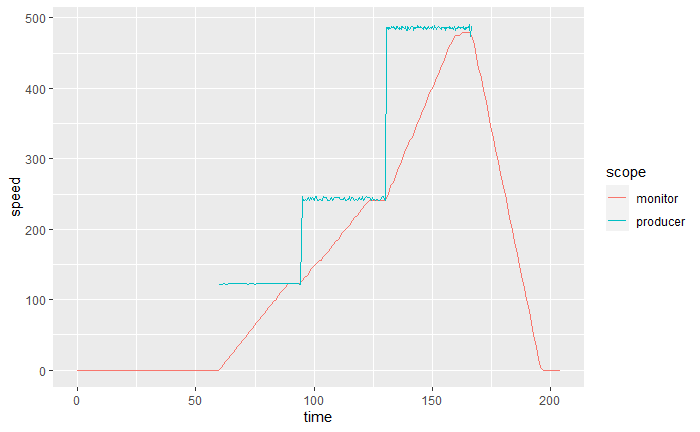
\includegraphics[width=0.7\textwidth]{images/monitor/monitor_step.png}
\caption{Monitor step response to three different controlled write speeds.}
\label{fig:monitor_step} \end{figure}

The second scenario has the producer wait a randomized time interval (between
$0.01s$ and $2s$) before sending the message to the partition. Since the monitor
takes into consideration the last $30s$ since it's latest measurement, it is not
affected by the noisy write speed as measured from the producer. Since the
implementation has the time interval as a uniform random variable, when the
monitor process stabilizes, it should stabilize on a speed rate as computed
using the time interval's expected value which is $\approx 1s$. This is in fact
the case as can be seen in \ref{fig:monitor_random}, since the write speed
stabilizes around $123 bytes/s$. The statistical description of the producer's
measured write speed better illustrates the noise reduction due to the monitor
computing the average over the last $30s$ of each measurement.

\begin{figure}[H] 
    \centering
    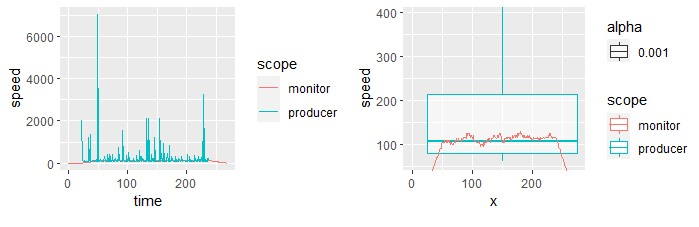
\includegraphics[width=\textwidth]{images/monitor/monitor_random.jpg}
    \caption{
        Monitor response to a producer waiting uniformely between [0.01,2]s
        every time it produces a record.
    } 
    \label{fig:monitor_random} 
\end{figure}


\section{Consumer} \label{component:consumer}

The Consumer goes through four important phases within it's process, to
approximate it's consumption rate to a constant value when being challenged to
work at it's peak performance. These phases repeat cyclically until the consumer
is terminated by an external termination signal, or in the event of an
unexpected exception. 

\subsection{Phase 1: Gathering Records}

The first phase is where data is gathered before being sent to the data
warehouse. 

The consumer is configured with two important parameters,
\lstinline[language=Python]{BATCH_BYTES} and
\lstinline[language=Python]{WAIT_TIME_SECS}, which indicate respectively, the
amount of bytes the consumer waits to gather in a single iteration, and the
amount of time it is allowed to wait to gather the information.

\subsection{Phase 2: Processing} \label{consumer:phase2}

\IncMargin{1em} \begin{algorithm}[h]
    \SetKwData{Left}{left}\SetKwData{This}{this}\SetKwData{Up}{up}
    \SetKwFunction{Union}{Union}\SetKwFunction{FindCompress}{FindCompress}
    \SetKwInOut{Input}{input}\SetKwInOut{Output}{output} \Input{\\ messages -
    List of Kafka messages,\\ mapTopicsTable - Map that indicates which table a
    message from a topic is inserted into } \Output{List<BatchList>} \BlankLine

mapTableBatchlist $\leftarrow$ new Map[String, BatchList]()\; \For{msg in
    messages}{ table $\leftarrow$ mapTopicTable.get(msg.topic())\; batchList
    $\leftarrow$ mapTableBatchlist.get(table)\; \If{(batchList == None)} {
        mapTableBatchlist[table] $\leftarrow$ new BatchList()\; batchList
$\leftarrow$ mapTableBatchlist.get(table)\; } batchList.add(msg)\; }
\KwRet{mapTableBatchlist.values()} \caption{Consumer Phase 2 algorithm}
\label{algo:phase_2} \end{algorithm}\DecMargin{1em}

The second phase is where the data gathered in the previous phase is prepared to
be sent into bigquery. Each record fetched from a Kafka topic, represents a new
row in a bigquery table. 

To insert data into bigquery, Google's Python Bigquery Client is used. Each post
request made with this client, has a batch of rows sent to a single table, and
it is also limited to no more than 10MB per request.

Since the gathered records originate from multiple topics, each row has to be
batched with data of it's kind, which are rows that are intended to be sent to
the same bigquery table.

A single instance of a Batch, a data structure created to agglomerate rows
intended for the same bigquery table, holds all the rows which will be sent in a
single post request through Google's python bigquery client API. Due to the
imposed limit of a post request, a Batch has a payload limit of $5 Mbytes$. 

A BatchList, is another data structure created to group instances of type Batch
that refer to the same table.

To process the data, a map stores the link between a table's id and the
BatchList instance assigned to it. When analyzing a message, it's topic metadata
indicates which table it is directed to, which in turn points to the BatchList
it must be added to.

When adding a message to a BatchList instance, this class controls to which
Batch it is assigned, based on the size of the row, and the size of the last
created Batch within this data structure.

\subsection{Phase 3: Sending Data into Bigquery}

This is the final stage of the consumer's insert cycle. There is a list of
BatchList instances, each having to be sent to a single bigquery table. To
optimize the insert cycle, this phase is done asynchronously with respect to all
the batches within the list of BatchLists contained in the map specified in
\ref{consumer:phase2}. In other words, each batch corresponds to an asynchronous
request to insert rows into a table.

After successful insert of the rows into the bigquery table, the messages are
then committed to Kafka. 

\subsection{Phase 4: Consumer Metadata}

\IncMargin{1em} \begin{algorithm}[h]
    \SetKwData{Left}{left}\SetKwData{This}{this}\SetKwData{Up}{up}
    \SetKwFunction{Union}{Union}\SetKwFunction{FindCompress}{FindCompress}
    \SetKwInOut{Output}{output}\SetKwInOut{Input}{input} \Input{consumer -
    consumer instance used to fetch information from the Kafka topics.}
    \Output{} \BlankLine

Set<Partition> current $\gets$ consumer.getCurrentState()\; Set<Partition>
    future $\gets$ current.copy()\;

Queue< Set<Partition> > changeStateQueue $\gets$ consumer.consumeMetadata()\;
    \While{changeState $\gets$ changeStateQueue.pop()}{ \eIf{changeState.type ==
    "StopConsumingCommand"}{ future $\gets$ future - changeState.partitions\; }{
        future $\gets$ future $\cup$ changeState.partitions\; } } toAssign
    $\gets$ future - current\; \label{algo:phase_4_toAssign} toStop $\gets$
    current - future\; consumer.incrementalAssign(toAssign)\;
    consumer.incrementalUnassign(toStop)\;
    \label{algo:phase_4_incremental_assign}

\caption{Consumer Phase 4 algorithm} \label{algo:phase_4}
\end{algorithm}\DecMargin{1em}

The consumer has to be informed by the Controller \ref{component:controller}, as
to which partitions it gets data from. For this purpose, to allow both the
controller and the consumers to work asynchronously, a message queue is the
ideal structure for this purpose.

Following event sourcing patterns, the current state of a single consumer should
be attained by consuming every message that was directed to it, which enforced a
change in state. With a slight modification, Kafka is used for this
communication between the controller and the consumers by creating a single
controller topic named \lstinline[language=Python]{data-engineering-controller}.

Maximum efficiency in data conveyed between each process, occurs when a single
process only reads messages which are relevant for it's functioning, without
having to ignore messages or data that it receives. As such, each consumer has
to be assigned a separate queue in the
\lstinline[language=Python]{data-engineering-controller} topic, which in Kafka
represents a distinct partition per consumer.

As will be further described in \ref{component:controller}, the consumer knows
which partition to consume from through it's deployment's name. When the
controller desires to communicate with this consumer, it simply has to send a
record to it's partition. 

Each record published into this topic has to have the same AVRO schema as
specified by \ref{appendix:avro_schema}. A command can be either a:
\begin{itemize} \item StartConsumingCommand - The consumer is to start consuming
            from each of the partitions within the record.  \item
StopConsumingCommand - The consumer stops consuming from the partitions
specified in the record.  \end{itemize}

The fourth phase starts with the consumer determining whether there are any
messages in it's metadata queue (the partition it was assigned from the
\lstinline[language=Python]{data-engineering-controller} topic). If there are
none, the consumer's state isn't changed, and the phase is finalized. Otherwise,
if there are any messages in the queue, the consumer goes through the process of
consuming all the messages in the metadata partition, and adds them to a Queue
instance \lstinline[language=Python]{changeStateQueue}.

The next step is to process the \lstinline[language=Python]{changeStateQueue}.
Initially, a set is created where each element represents a partition from a
topic the consumer is currently consuming from. This set is stored in the
variable \lstinline[language=Python]{current}. A copy of this set is made and
assigned to a variable \lstinline[language=Python]{future}. While the queue is
not empty, the front-most element is removed and assigned to a temporary
variable \lstinline[language=Python]{changeState}. Depending on the command, if
the record requests the consumer to start consuming from it's set of partitions
then a union operation is performed between the
\lstinline[language=Python]{future} and the
\lstinline[language=Python]{changeState}. In turn, if the record is of type
"StartConsumingCommand", the difference between future and change state is
computed.

Having processed the whole \lstinline[language=Python]{changeStateQueue}, future
holds the new state the consumer has to change into. Lines
\ref{algo:phase_4_toAssign} to \ref{algo:phase_4_incremental_assign} change the
consumer's assignment into future's state.

\subsubsection{Persisting Metadata}

The final stage of the consumer goes through persisting the consumer's metadata
in case the consumer fails and has to pick up the work it was last performing.
The data to be persisted is the set of partitions it is currently consuming
from. This means that a successful change in consumer metadata would only occur
after the consumer successfully persists the data to it's persistent volume.

Since the consumer is a pod within a deployment in a Kubernetes cluster, the
container responsible for this component starts with a clean slate. When the
container is terminated the data written to disk is cleaned,  making it
inaccessible for future reads outside of a single pods lifetime. This type of
storage is named ephemeral as it has the same lifetime as the pod.

Kubernetes provides with volumes which can be of type ephemeral or persistent
(it's lifetime is independent of the pod's). 

A persistent volume (PV) can be created static or dynamically, and is a resource
within the cluster. A persistent volume claim (PVC), is a method of abstraction
which allows a user to request for storage. This request, then tries to match
the claim to one of the available resources, and if there are none available,
then a new persistent volume can be created dynamically if the Storage Class is
defined. The mapping between PV and PVC is one-to-one.

This consumer uses both types of volumes, since the downwardAPI is of type
ephemeral and it provides the consumer with it's context, giving it access to
it's deployment's name (data the consumer requires for it to know which
partition to consume from in the data-engineering-controller [metadata] topic).
As for the persistent volume, the consumer will use this type of volume to
persist the data for it's current consumption state.

If the consumer fails unexpectedly, then on startup, it just has to verify it's
state on the volume, and in case it was performing any tasks, it picks up where
it left off.

When stopping a consumer, to safely terminate it's tasks, the controller sends a
StopConsumingCommand for all the partitions the consumer is currently assigned
to. After the consumer acknowledges it acted to the command (it sends a
StopConsumingEvent back to the controller
\ref{sub:controller_communication_cosumer}), the controller then terminates the
pod. The fact termination only occurs after the consumer updates it's metadata,
implies the persistent volume is also updated to an empty set, which allows a
new consumer of the same deployment to start off with a clean slate as should be
the case, since the consumer was gracefully terminated.


\subsection{Consumer Maximum Capacity}
\label{c3subsub:consumer_maximum_capacity}

The way the problem is formulated assumes the consumer is capable, when
required, to achieve a maximum data consumption rate, still to be defined,
analogous to the capacity of a bin in a BPP.

With the goal of attaining a value for this maximum bin capacity, the consumer
was tested in 3 different scenarios, each requiring the consumer to be working
at peak performance.

Peak performance is defined as the case when the sum of the bytes still to be
consumed from all the partitions the consumer is assigned to, is bigger than
\lstinline[language=Python]{BATCH_BYTES}.

The 3 testing scenarios aim to test the consumer's throughput while varying the
number of tables it has to insert data into, the average amount of bytes
available in each of the assigned partitions, and the number of partitions
assigned to it.

The consequence of having more tables where data has to be inserted, directly
affects the third phase by increasing the amount of asynchronous request that
have to be made.

As for reducing the average amount of bytes available in the partitions
assigned, but still being able to make the consumer work at full capacity, aims
to test the first phase of the algorithm, where the data has to be consumed from
the partitions assigned from Kafka.

This is the case since this high-level consumer is based on the Kafka client
provided by the confluent\_kafka package. When the client begins, it starts a
low level consumer implemented in C that runs in the background. As the
low-level consumer runs, it buffers messages into a queue until the high level
python consumer requests for what it has consumed with either
\lstinline[language=Python]{poll()} or the
\lstinline[language=Python]{consume()} methods. The difference between these two
methods is that the first returns a single message whereas the second returns a
batch of messages defined by \lstinline[language=Python]{num_messages}, from the
kafka client's buffer. 

To improve throughput, when a consumer requests for data from the broker, the
broker attempts to batch data together before sending it back to the consumer.
\lstinline[language=Python]{fetch.max.bytes} and
\lstinline[language=Python]{fetch.max.wait.ms} define how a single request is
handled by the broker, wherein the first determines the maximum amount of bytes
returned by the broker, and the second, the amount of time the broker can wait
before returning the data if fetch.max.bytes is not satisfied.

Reducing the average amount of bytes in each of the partitions assigned, leads
to the consumer having to perform more requests to fetch the same amount of data
defined by \lstinline[language=Python]{BATCH_BYTES}. 

The number of partitions assigned to the consumer is expected to influence the
time it takes for the consumer to gather
\lstinline[language=Python]{BATCH_BYTES}, by increasing the amount of requests
required to fetch the data, as assigning partitions increases the probability of
the consumer having to communicate with more brokers. 

Another important definition is that the consumer is said to have reached it's
steady state, when it is capable of fetching
\lstinline[language=Python]{BATCH_BYTES} prior to
\lstinline[language=Python]{WAIT_TIME_SECS} being triggered in it's first phase.
This reflects that the low-level consumer is capable of gathering the necessary
amount of bytes into it's buffer, while the high-level consumer is running all
the remaining phases except the first of the insert cycle.

For the following test cases, \lstinline[language=Python]{BATCH_BYTES = 5000000}
and \lstinline[language=Python]{WAIT_TIME_SECS = 1}.

These values inherently reflect the time it takes for a consumer to go through
each of it's phases, and the rate at which it can consume data.

\begin{table}[H] \centering \caption{Testing conditions to obtain consumer
    maximum throughput measure.} \begin{tabular}{ |c|r|r|r|r| } \hline
        \textbf{Test ID} & \textbf{Total Bytes} & \textbf{Average Bytes} &
        \textbf{Number of Partitions} & \textbf{Number of Tables} \\ \hline Test
    1 & $648058050$ & $20251814$ & $32$ & $1$ \\ Test 2 & $100140747$ & $863282$
    & $116$ & $5$ \\ Test 3 & $678388069$ & $4711028$ & $144$ & $5$ \\ \hline
    \end{tabular} \end{table}

Test 1 has the consumer fetching records which are all directed to the same
    table, and every partition it visits has enough bytes to satisfy the
    max.fetch.bytes condition, optimizing the throughput between the low-level
    consumer and the brokers, as the data is batched together. Since there is
    only one table to send the data to, the third phase is also optimized as
    there will only be a single BatchList instance.

As for Test 2, the increased number of partitions and the reduced average amount
    of bytes in each partition has the consumer polling more brokers to gather
    \lstinline[language=Python]{BATCH_BYTES}, increasing the time the consumer
    takes in the first phase. Although the time taken in this phase increased
    The average time it takes the consumer to fetch
    \lstinline[language=Python]{BATCH_BYTES} from the kafka cluster, indicates
    that the consumer still manages to reach its steady state.

Lastly, Test 3 combines both of the previous scenarios, where there is more data
    per partition to be sent back to the consumer, although some iterations
    require the consumer to send data to 5 different tables since the data
    originates from partitions that belong to different topics.

The metrics that were deemed important for the analysis of the consumer's
    behaviour, were: Time to go through Phase 1 ($\Delta t_{P1}$); Time to go
    through Phase 2 ($\Delta t_{P2}$); Time to go through Phase 3 ($\Delta
    t_{P3}$); Total cycle time ($\Delta t$); Measured cycle throughput.

Each of these parameters is statistically summarized in the following table:
    \begin{table}[H] \centering \caption{Statistical summary of the metrics }
        \begin{tabular}{ |c|l|r|r|r|r|r| } \hline \textbf{Test ID} &
            \textbf{Summary Measure} & \textbf{$\Delta t_{P1}$} &
            \textbf{$\Delta t_{P2}$} & \textbf{$\Delta t_{P3}$} &
            \textbf{$\Delta t$} & \textbf{Throughput} \\ \hline
            \multirow{2}{*}{Test 1} & Average            & 0.394  & 0.000775 &
            1.69   & 2.08 &                              2417215.33 \\ &
            Standard Deviation & 0.0338 & 0.00620  & 0.0941 & 0.101 & 99234.23
            \\ \hline \multirow{2}{*}{Test 2} & Average            & 0.462  &
            0.00684 & 1.72 & 2.18 &                                 2307501.21
            \\ &  Standard Deviation & 0.125 & 0.001600  & 0.0946 & 0.169 &
            171231.27 \\ \hline \multirow{2}{*}{Test 3} & Average            &
            0.397  & 0.00896 & 1.68   & 2.08 &
            4218220.20 \\ &  Standard Deviation & 0.0466 & 0.00619  & 0.105 &
        0.121 & 132017.37 \\ \hline \end{tabular} \end{table}

The following graph demonstrates how the consumer is capable of maintaining a
        stable speed above a threshold of $2 Mbytes/s$, when it finds itself in
        it's steady state (capable of consuming $5 Mbytes$ before
        \lstinline[language=Python]{WAIT_TIME_SECS} is triggered), sharing a
        mode between the three different testing scenarios around $2.3
        Mbytes/s$.

\begin{figure}[H] \centering
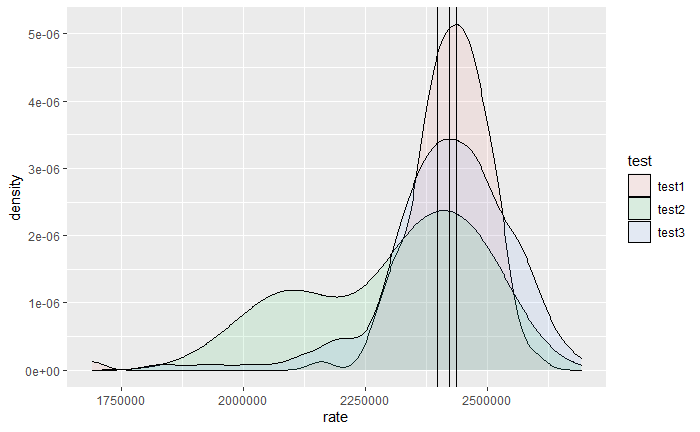
\includegraphics[width=\textwidth]{images/consumer/Consumer_Capacity.png}
\caption{Density Plot for the consumer's measured throughput in the 3 testing
conditions.} \label{fig:consumer_capacity} \end{figure}

\subsubsection{Bin Capacity} \label{result:bin capacity}

Two measures are defined which are to be used in the sections to come. The
        \lstinline[language=Python]{ALGORITHM_CAPACITY}, is the constant bin
        size that will be used when running all the heuristic algorithms when
        solving the dynamic BPP, whereas the
        \lstinline[language=Python]{CONSUMER_CAPACITY} is the consumer's maximum
        capacity, which if exceeded, must trigger a new configuration as for
        which partition should be assigned to which consumers.

The reason for having defined these two configuration parameters differently are
        due to the problem's dynamic nature. Since the measured write speed for
        each partition varies between each measurement, after executing the BPP
        algorithm for a single measurement, it is common to have bin's filled
        close to their capacity, which would lead to excessive rebalancing
        computations if the algorithm and consumer capacity were defined using
        the same value. Defining the Consumer's capacity to a value higher than
        the algorithm's perceived capacity, reduces the number of rebalances
        triggered, but also at the cost of the each configuration having more
        consumers than required. 

From the graph \ref{fig:consumer_capacity}, the Consumer's capacity is set to $2
        Mbytes$, whereas the Algorithm's capacity is defined as $1.5 Mbytes$.
        These are the values used for the remaining part of the work.

It is important to note that these values are only valid when the consumers are
        deployed in the environment where they were tested. As long as the
        consumers share the same stable environment, the maximum capacity does
        not change with the parameters previously mentioned, and therefore the
        test can be run again to get these same baseline values. 

\section{Controller/Orchestrator} \label{component:controller}

The controller is the component of the system which is responsible for
orchestrating and managing the consumer group that is intended to consume the
data from the partitions of interest. 

The problem is modeled as a dynamic bin packing problem, where the size of each
item is equivalent to the write speed of each partition, and the size of the
container represents the maximum achievable speed of a consumer which has been
provided by the data presented in \ref{result:bin capacity}.

For clarity, for the following sections, consumer, container and bin will be
used interchangeably, representing a consumer instance described in
\ref{component:consumer}.

This problem is different to the usual bin packing problem due to the changing
write speed of each partition (the size of the items). This implies that a
viable solution in one iteration, might not be viable in a future iteration when
the sizes have changed.

At any given time, no consumer within the consumer group can have it's capacity
exceeded by the cumulative write speed of the partitions assigned to it, and if
it is, then a rebalance has to be triggered. The same applies in case a
partition has not yet been assigned a consumer.

After the controller determines the state in which it wants its consumer group,
it then creates the consumers that don't yet exist, communicates the change in
assignment to each consumer in the group, followed by deleting the consumers
that are not required in the new computed group's state.

While rebalancing any partition, during the time the controller is informing the
current consumer to stop reading from it to inform the new consumer to start
doing so, the messages belonging to this partition are not being read. This is
the new cost that has to be taken into consideration when dealing with the
rebalancing procedure.

\subsection{System Design}

As has been described, there are three different components in the system that
work together to get the data from Kafka into bigquery. To do so, each component
has to be able to communicate with one another to inform any change in state. 

For this reason, the following diagram describes how the pieces fit together,
and communicate with one another.

\begin{figure}[H] \centering
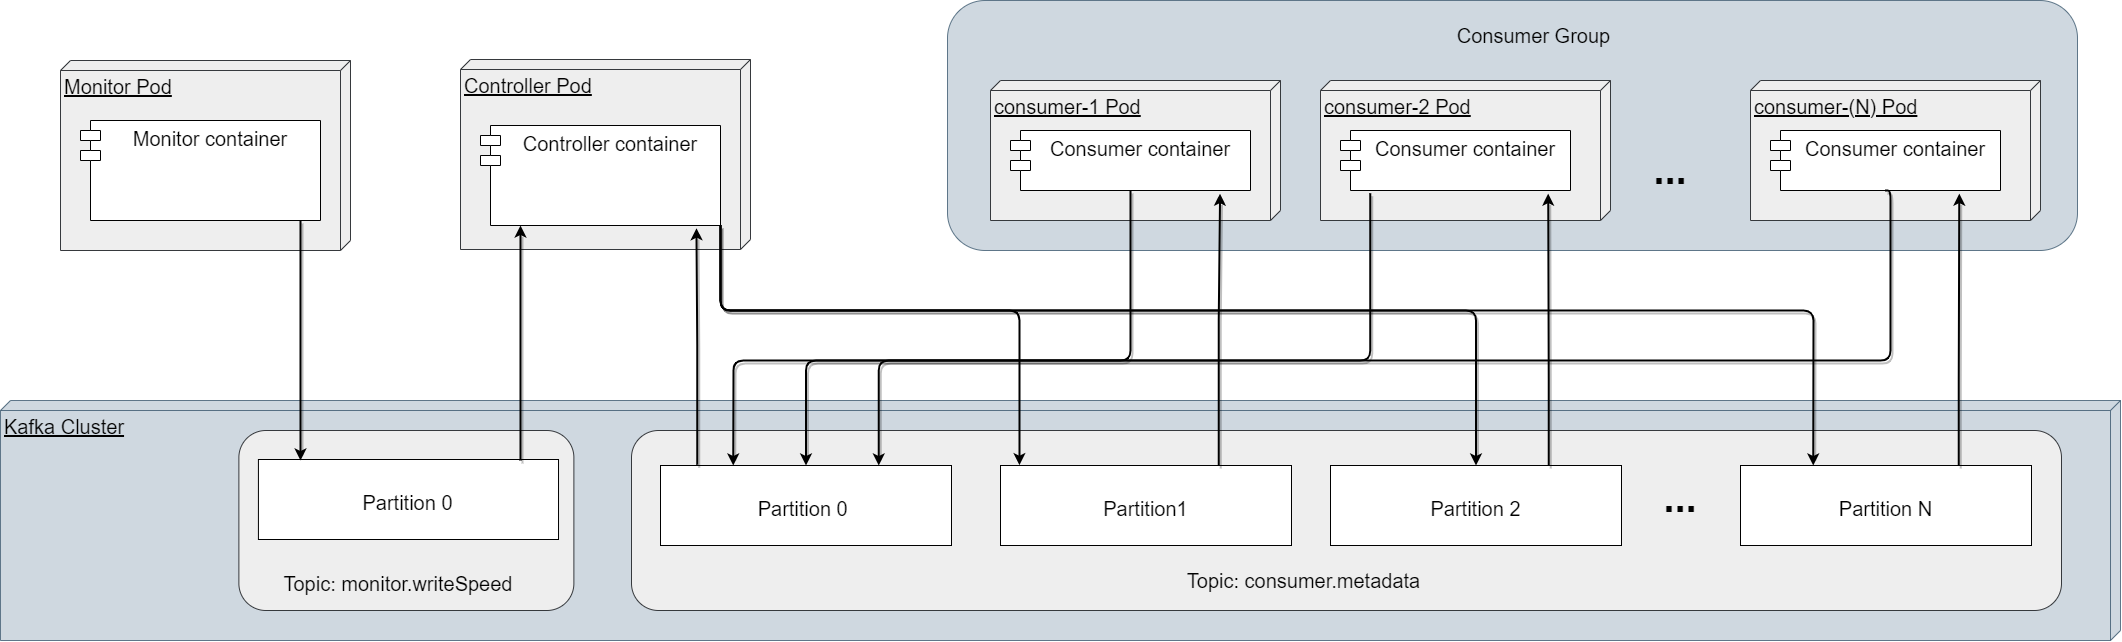
\includegraphics[width=\textwidth]{images/controller/System Design.png}
\caption{System architecture deployment diagram} \label{fig:system_architecture}
\end{figure}

As shown in the diagram, there are two main topics that will be responsible for
providing an asynchronous communication between the 3 different entities of the
system. The data-engineering-monitor topic, is where the monitor process sends
the speed measurements for the controller to consult, whereas the
data-engineering-controller topic is where the controller sends messages to each
consumer to inform the change in their state. Partition 0 of this topic is
reserved for the controller so the consumers always know how to acknowledge
their change in state.

When using a Kafka topic to communicate between the consumers and the controller
there are certain requirements that need to be complied with. 

The first, is that when the controller communicates with a consumer from the
consumer group, it has to be guaranteed that the message reaches the intended
consumer. 

Secondly, as will be common with this system, the controller will create and
delete a single consumer multiple times in its lifecycle. The message offset a
consumer starts on after restarting, has to be precisely the one where it left
off before being shut down by the controller. This can be done leveraging
kafka's \lstinline[language=Python]{group-id} property, defined in each consumer
client, and so the system just has to guarantee that the consumer gets the same
id as before.

Thirdly, each consumer only reads messages which are intended to it. This would
represent maximum efficiency in the information transmitted between both
controller and consumer, since no process is reading messages that have to be
ignored. To better understand this design requirement, the following scenario is
described: It might happen that a certain number of consumers satisfies the
controller's conditions, without any need to scale up or down the group. This
would imply that the control messages sent by the controller are only read by
the currently active consumers. When a new consumer is started by the
controller, if the messages are shared, then there is a big queue of messages
that have not yet been read by the new consumer since it was last up. For the
new consumer to be able to read new control messages sent by the controller, it
would first have to read all messages that were not intended to it prior to it
starting up.

Lastly, to guarantee temporal consistency in the control messages sent to a
single consumer, it is clear that a control message can only be sent to a single
partition, as kafka only guarantees message read order when the messages belong
to the same partition. Kafka already does this by allowing a message to have a
key attribute which is then hashed to determine the partition in which the
message is to be inserted. The issue with this approach is if the number of
partitions in the data-engineering-controller topic increases, the key might not
send the messages to the same partition as before. As such, each consumer is
given an incremental id ($1, 2, ...$), which represents the partition where
change in state information has to be sent for the consumer to read (both
controller and consumer are aware of this id).

\subsection{State Machine}

The controller can be defined by a state machine, intended to continuously
manage a group of consumers and their assignments. A group's assignment
represents the same group's state.

The following diagram shows the high level architecture of the controller
process:

\begin{figure}[H] \centering
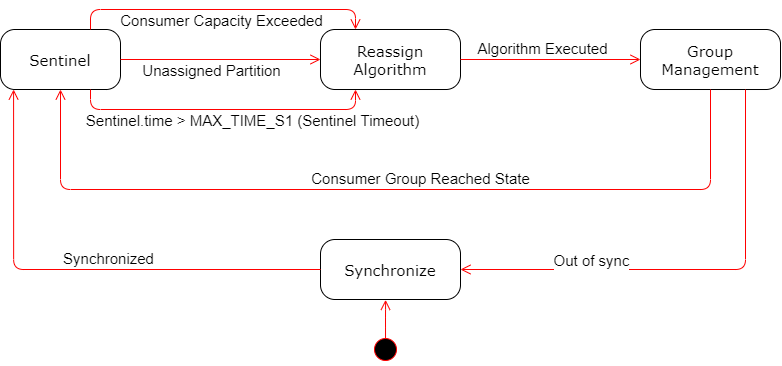
\includegraphics[width=\textwidth]{images/controller/state_machine.png}
\caption{Controller State Machine.} \label{fig:state_machine} \end{figure}

\subsection{State Sentinel}

This state is where the controller uses the information provided by the monitor
component (\ref{component:Monitor}), to determine whether it has to recompute
the consumer group's assignment. The first step the controller goes through in
this state is to read the last speed measurement the monitor component added to
the data-engineering-monitor topic.

The controller then updates each of the partition's speeds, which in turn
updates the cumulative speed of each consumer. As can be seen in figure
\ref{fig:state_machine}, there are three transitions that can lead to the
controller re-computing the current consumer group's assignment:
\begin{enumerate} \item \textbf{Consumer Capacity Exceeded} - This transition is
        triggered if the cumulative speed of all the partitions assigned to any
    consumer, exceeds the maximum consumer capacity measured in \ref{result:bin
capacity}.  \item \textbf{Unassigned Partition} - If there is any partition
    within the last speed measurement that is not currently assigned to a
        consumer, then this transition is triggered.  \item \textbf{Sentinel
            Timeout} - One of the controller's configurations, is a parameter
            \lstinline[language=Python]{MAX_S1_TIME} which indicates the maximum
            amount of time the controller can spend in the sentinel state
            without triggering a rebalance. This trigger is to have a condition
            that runs the algorithm to verify if downscaling is viable, as the
            other triggers are directed to upscaling conditions.
\end{enumerate}

\subsection{State Reassign Algorithm}

This state receives as input the current consumer group's assignment and the
remaining unassigned partitions, and produces as output a new consumer group
assignment, which is to be defined as the group's future state.

This state uses only approximation algorithms to determine the group's future
assignment. The algorithms implemented are the already existing Next Fit, First
Fit, Worst Fit, Best Fit, and each of the previous algorithms' decreasing
versions, and modified versions of the Best and Worst Fit algorithms. 

In the implementation of the existing approximation algorithms, another step was
included during the creation of the bins which does not affect the outcome in
terms of number of consumers. If the consumer that is currently assigned to the
partition has not yet been created in the future assignment, this is the bin
that is created, otherwise, the lowest index bin that does not yet exist is the
one created.
 
\begin{figure}[H] \centering
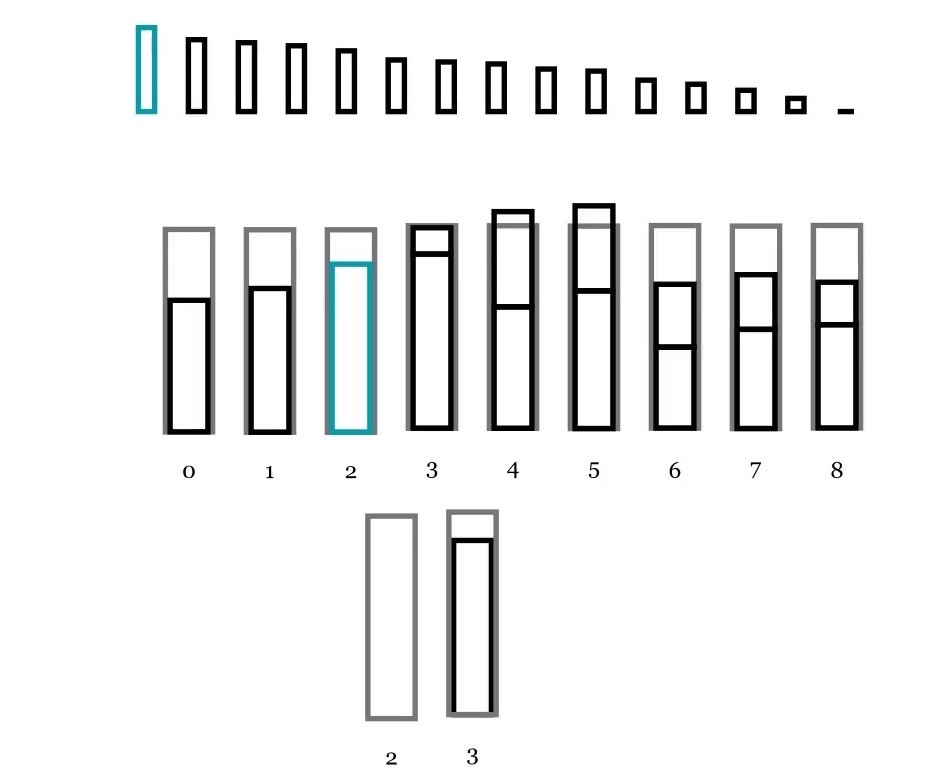
\includegraphics[width=0.6\textwidth]{images/controller/ApproximationAlgorithm_NewBin.png}
\caption{New bin creation procedure when performing an approximation algorithm.}
\label{fig:approximation_bin_creation} \end{figure}

Figure \ref{fig:approximation_bin_creation} illustrates this process, wherein
the first row of consumer's (grey containers) represents the current consumer
group's state, and the second the new consumer group assignment that is being
computed by the controller. Partitions are represented in red and white, red
being the partition currently being analyzed by the controller. In this example,
the red partition currently finds itself in the consumer 2. When analysing the
partition, the controller verifies if the partition fits in any of the existing
partitions. Since it does not fit, and another consumer has to be created for
this partition, the new consumer is the same as the one it is currently
assigned, therefore occurring no rebalance for this partition.

This is not presented as a modification to these algorithms as their
functionality does not change with this approach to for a bin's creation, as it
simply adapts the algorithms to the rebalancing problem at hand, improving it as
compared to always creating the lowest index bin, as that would imply
rebalancing partitions more often.

\subsubsection{Modified Any Fit Algorithms}
\label{subsub:modified_any_fit}

The motivation to modifying the existing Any Fit algorithms, is that the item
reassignment is not the problem they are trying to solve, they simply aim to
reduce the amount of active bins for a certain list of items. 

Within this problem's context, rebalancing inevitably implies having the
consumer group to stop consuming from a partition, while the controller is
reassigning the partition from one consumer to another (as there cannot be a
concurrent read from the same partition).

A new measure is presented to compute the the total rebalance cost (Rscore), of
a new group's configuration. This metric represents the rate at which
information is accumulating for each second that passes, given in consumer
iterations per second.

\begin{table}[H] \centering \caption{Data to compute the Rscore for an
    iteration.} \begin{tabular}{ |c|l| } \hline \textbf{Symbol} &
        \textbf{Description} \\ \hline $P_i$ & set of partitions that were
        rebalanced in iteration $i$ \\ $s(p)$ & outputs the write speed of
        partition $p$ \\ $R_i$  & Computed total Rscore for iteration $i$ \\ $C$
    &  Constant that represents the maximum consumer capacity from
    \ref{result:bin capacity}\\ \hline \end{tabular} \end{table}

The following equation then presents the cost of rebalancing for a single
    iteration $i$.

\begin{equation} R_i = \frac{1}{C}\sum_{p \in P_i} s(p) \end{equation}

Since the controller has access to the speed measurements of all partitions and
    it does not require to read and assign each partition in any particular
    order, this bin packing problem can be categorized as offline.

Different from the previous decreasing versions of the Any Fit algorithms which
    have already been described in \ref{sub:Approximation Algorithms and
    Heuristics}, this algorithm will not sort the partitions, but in turn the
    consumers (bins).

There will be 2 main approaches to sorting the consumers: \begin{itemize} \item
        Sorting each consumer based on their current cumulative speed
    (cumulative sort); \item Sorting each consumer based on the partition
        assigned to it that has the biggest measured write speed (max partition
        sort).  \end{itemize}

After sorting the current consumer group using one of the above strategies, the
    procedure is as follows:

\IncMargin{1em} \begin{algorithm}[h]
    \SetKwData{Left}{left}\SetKwData{This}{this}\SetKwData{Up}{up}
    \SetKwFunction{Union}{Union}\SetKwFunction{FindCompress}{FindCompress}
    \SetKwInOut{Input}{input}\SetKwInOut{Output}{output} \Input{current consumer
    group C and set of unassigned partitions U} \Output{consumer group N which
    is the next state for the consumer group} \BlankLine N $\leftarrow$ new
    ConsumerList(assign\_strategy=("BF" | "WF"))\; sorted\_group $\leftarrow$
    sort(C, sort\_strategy=("cumulative" | "max partition"))\; \For{consumer
    $\in$ sorted\_group}{ Set<Partition> partitions $\gets$
    consumer.assignedPartitions()\; List<Partition> sorted\_partitions
    $\leftarrow$ sort(partitions, reverse=True)\; \For{i $\leftarrow$
    length(sorted\_partitions)-1 \KwTo 0}{ partition $\leftarrow$
    sorted\_partitions[i]\; result $\leftarrow$ assignExisting(N, partition)\;
    \If{result $==$ False}{ break\; } remove(sorted\_partitions, partition)\; }
    \If{sorted\_partitions.length() == 0}{ continue\; } createConsumer(N,
    consumer)\; \For{partition $\in$ sorted\_partitions}{ result $\leftarrow$
    assignCurrent(N, partition, consumer)\; \If{result $==$ False}{ break\; }
    remove(sorted\_partitions, partition)\; } extend(U, sorted\_partitions)\; }
    sorted\_unassigned $\leftarrow$ sort(U, reverse=True)\; \For{partition $\in$
    sorted\_unassigned}{ assign(N, partition)\; } \KwRet{N} \caption{Modified
Any Fit Pseudo Code}\label{algo:MBPP} \end{algorithm}\DecMargin{1em}


For each consumer in the sorted consumer group, the partitions assigned to the
    consumer are sorted based on their write speed. From smallest to biggest,
    each partition is inserted into one of the bins that have already been
    created in the future assignment, based on one of the any fit strategies,
    which in the tested implementation, can either be with a Best or Worst Fit
    strategy. If the insert is successful, then the partition is removed from
    the sorted list of partitions, otherwise, if there is no existing bin that
    can hold the partition, then the current consumer assigned to it is created. 

The remaining partitions in the sorted list are now inserted into the newly
created bin, from biggest to smallest, and removed from the sorted list if
successful. If a partition does not fit into the newly created consumer, then
the remaining partitions in the list of sorted partitions are added to the set
of unassigned partitions.

After performing the same procedure over all consumers, there is now a set of
partitions which have not been assigned to any of the consumers in the future
assignment. These partitions are first sorted in decreasing order (based on
their measured write speed), and each partition is assigned using their
respective any fit strategy.

\begin{table}[H] \centering \caption{Modified implementations of the any fit
    algorithms.} \begin{tabular}{ |c|c|c| } \hline \textbf{Algorithm} &
        \textbf{Assign Strategy} & \textbf{Consumer Sorting Strategy} \\ \hline
        Modified Worst Fit & Worst Fit & cumulative write speed \\ Modified Best
        Fit & Best Fit & cumulative write speed \\ Modified Worst Fit Partition
        & Worst Fit & biggest partition write speed \\ Modified Best Fit
        Partition &  Best Fit & biggest partition write speed \\ \hline
    \end{tabular} \end{table}

\subsubsection{Testing} \label{c3subsub:testing}

To evaluate the performance of each of these algorithms, two metrics were used:
    The relative difference in the number of consumers of each algorithm to the
    approximation algorithm that presented the least amount of consumers; The
    Rscore of the algorithm's new configuration.

\begin{table}[H] \centering \caption{Data to create the testing environment for
    the approximation algorithms.} \label{table:testing_data} \begin{tabular}{
            |c|l| } \hline \textbf{Symbol} & \textbf{Description} \\ \hline $P$
        & Set of partitions assigned to the consumer group. \\ $s_p^i$ &
    Provides the speed for partition $p$ in iteration $i$ \\ $\phi(\delta)$ &
    Uniform random function that selects a value between $[-\delta, \delta]$\\
    \hline \end{tabular} \end{table}

Given the data provided by \ref{table:testing_data}, the testing sequences for
the algorithms was obtained as follows: \begin{enumerate} \item 200 different
            partitions are created and given an initial speed. Four different
            initial conditions for all partition were tested: Starting at $0\%$
            of the \lstinline[language=Python]{ALGORITHM_CAPACITY}; Starting at
            $50\%$ of the \lstinline[language=Python]{ALGORITHM_CAPACITY};
            Starting at $100\%$ of the
            \lstinline[language=Python]{ALGORITHM_CAPACITY}; Assigning each
            partition a uniform random value between $[0, 100]\%$ of the
            \lstinline[language=Python]{ALGORITHM_CAPACITY}.
    
    \item Given the initial conditions, a new measurement is created, where the
        speed in the next measurement is calculated using: \begin{equation}
        s_p^{i+1} = s_p^i + \phi(\delta) \times algorithm\_capacity, \quad
        \forall p \in P, \end{equation} having $\phi(\delta)$ be evaluated every
        new computation.
    
    \item The previous step is repeated for the next measurements until there
are 500 measurements in a single sequence.  \end{enumerate}

Using this procedure, six different sequences of measurements were created, each
    differing in the $\delta$ used to vary the speed. As such, for each initial
    condition, there is a sequence where $\delta$ is set to $0, 5, 10, 15, 20,
    25$. In other words, there are $6 (deltas) \times 4 (starting\; conditions)$
    different sequences, each representing a measurement instance provided by
    the monitor process. After reading a single measurement from a sequence, the
    controller runs the implemented algorithms to find the group's configuration
    in all scenarios.

\begin{figure}[H] \centering
    \includegraphics[width=0.8\textwidth]{images/controller/Relative Number of
    Consumers.png} \caption{Average Relative Deviation from the configuration
    that provides the minimum number of consumers, with a random initial speed
    for each partition.} \label{fig:relative_nconsumers} \end{figure}

To better illustrate the performance of the algorithms for each measurement
    sequence, the metrics are statistically summarized using the average. The x
    axes refers to the 6 different measurement sequences for a given starting
    condition, and the value is the $\delta$ defined for that measurement. As
    for the y axes in \ref{fig:relative_nconsumers}, it indicates the
    algorithm's average relative deviation from the configuration that provides
    the minimum number of consumers.

In \ref{fig:relative_nconsumers}, each partition starts with a random speed
    between $[0,100]\%$ of \lstinline[language=Python]{ALGORITHM_CAPACITY}. The
    worst performing algorithm is the next fit followed by it's decreasing
    version, since every time a partition is to be assigned, the algorithm only
    verifies if it fits in the last created bin, as opposed to considering all
    the already existing bins. The remaining any fit decreasing algorithms, are
    the ones that perform the best, with the best fit decreasing consistently
    presenting the best results. 

\begin{figure}[H] \centering
    \includegraphics[width=0.7\textwidth]{images/controller/Relative Number of
    Consumer Modified.png} \caption{Average Relative Deviation from the
    configuration that provides the minimum number of consumers, with a random
    initial speed for each partition. (Filtered to present the modified
    algorithms and BFD)} \label{fig:relative_nconsumers_modified} \end{figure}

As for the modified versions of these algorithms, due to its sorting strategy,
MBFP shows the best results. It is also worth noting that for smaller
variabilities, the modified algorithms behave similarly to the online versions
of their any fit strategy, but, the higher the delta, the bigger the
variability, which also leads to more rebalancing, having the modified
algorithms behave more like the decreasing versions of their fit strategy.

\begin{figure}[H] 
    \centering
    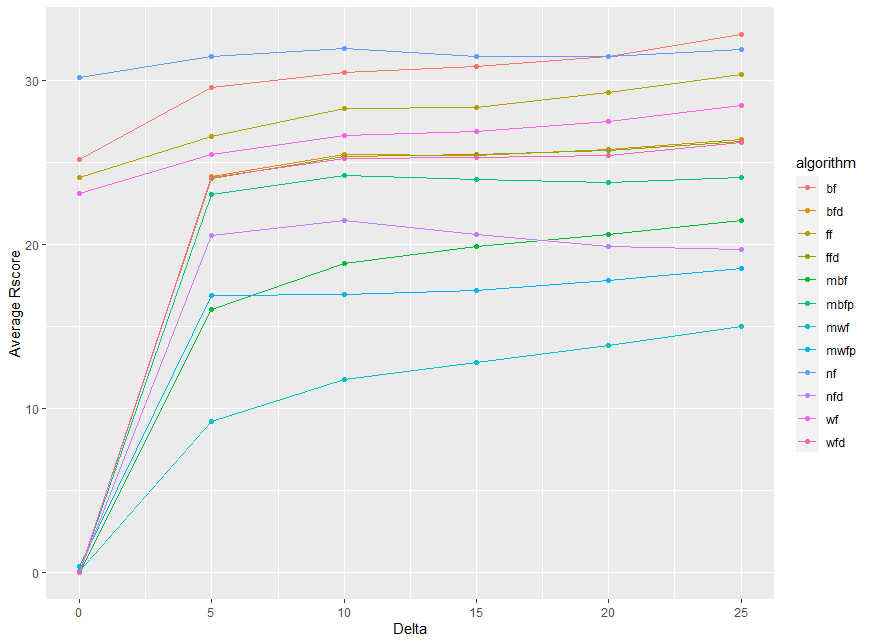
\includegraphics[width=0.7\textwidth]{images/controller/Rscore.png}
    \caption{
        Impact on Rscore for different Deltas (random initial partition speed).
    } 
    \label{fig:rscore} 
\end{figure}

For the same starting conditions, \ref{fig:rscore} presents the average Rscore
of each algorithm for all six measurement sequences.

As can be seen in \ref{fig:rscore}, the modified algorithms present the best
Rscore for each measurement along with next fit decreasing. The reason why the
NFD presents such a result, is due to the increased amount of consumers it
creates to assign new partitions, which at the moment of creation, will always
be the same consumer as the one assigned to the partition being analyzed, as
long as it has not yet been created (\ref{fig:approximation_bin_creation}).

For a similar reason, the modified algorithms that perform the best with regards
to the Rscore, are also the ones that perform worst (compared to the remaining
modified algorithms) when evaluating the relative number of consumers.

The remaining tests performed are presented in the appendix, and it can be
concluded, that the initial conditions do not significantly affect the relative
performance of the algorithms (\ref{}).

To select the algorithm to use within the controller, there is a trade-off
between the aforementioned testing metrics. On account of the added re-balance
concern within the modified algorithms, these present an improvement with
regards to the Rscore compared to the approximation algorithms presented in the
literature.

\begin{figure}[H] \centering
\includegraphics[width=\textwidth]{images/controller/Facet Wrap Pareto
Front.png} \caption{Pareto Front for each delta value used in the measurement
sequences.} \label{fig:pareto_front} \end{figure}

The pareto front is a way of evaluating the set of solutions that are most
efficient, provided there are trade-offs within a multi-optimization problem.

Excluding MWFP, the modified algorithms are consistently a part of the pareto
front \ref{fig:pareto_front}, which implies these are a competitive option as to
which algorithm to pick for the reassign algorithm to be executed in the
controller. The algorithm that shows the best Rscore for the different
variabilities is the MWF, whereas the modified algorithm that performs the best
relative to the number of consumers used in each configuration is the MBFP.

\subsection{State Group Management}

This state is where the controller informs each consumer of their change in
state. Since there cannot be any concurrent read of a partition by two consumers
of the same consumer group, when rebalancing a partition, the controller first
has to inform the consumer currently assigned to the partition to stop consuming
from it, and only after the consumer acknowledges having acted to the request,
can it inform the new consumer of it's new assignment.

This state not only handles this message exchange but it also creates and
deletes consumer resources from the Kubernetes cluster. 

\subsubsection{Difference between current and future state}

The current consumer group's state is represented by a list of consumers, each
having their own assignment. The new computed group's state is defined as the
next state, and is also a list of consumer's each having an assignment, but
representing the desired state the controller will communicate to each consumer.

Similar to computing the difference between two sets, when computing the
difference between 2 consumer lists the procedure involves iterating over each
consumer (in both states), and calculate the difference between the two consumer
assignments (set of assigned partitions). There are three scenarios that result
in different actions the controller has to perform, for a given position $i$ of
each consumer list: \begin{itemize} \item next state has a consumer at $i$ but
            the current state does not - This means that the consumer has to be
            created by the controller, and the partitions assigned to the
            consumer in position $i$ of the next state, have to be associated
            with a StartConsumingCommand for this same consumer.  \item next
                state does not have a consumer at $i$ but the current assignment
                does - The partitions associated with the consumer at position
                $i$ of the current state have to be associated with a
                StopConsumingCommand directed to this consumer, and the consumer
                has to be added to the list of consumers to remove.  \item both
                    next state and current state have a consumer at position $i$
                    - This means that no creation or deletion operation has to
                    be performed for this bin, and the operations to perform in
                    this case are only communicating to the already existing
                    consumer the difference in it's assignment. 
    
    The same consumer has two different sets of partitions assigned to it
        represented in the two different group states.
        \lstinline[language=Python]{next_assignment} will denote the set of
        partitions attributed to the consumer's state in the next group's
        context, and \lstinline[language=Python]{current_assignment} is defined
        as the consumer's set of partitions in it's current state.
    
    \begin{lstlisting}[language=Python] partitions_stop = current_assignment -
    next_assignment partitions_start = next_assignment - current_assignment
    \end{lstlisting} the resulting set of partitions within
        \lstinline[language=Python]{partitions_stop} have to included in a
        StopConsumingCommand, whereas the partitions in
        \lstinline[language=Python]{partitions_start} in a
        StartConsumingCommand, both message types directed to consumer $i$.
\end{itemize}

\subsubsection{Managing the Consumer Group in the Kubernetes Cluster}

Each active consumer in the current group's state, represents a deployment with
a single replica (pod). The reason why this is the case is that each consumer
requires a volume to persist its data, which implies having a different volume
for each pod. This is also possible using stateful sets, but the constraint of a
stateful set is that when removing a replica of the set, it only allows to
remove the last added replica, and in this context, a more granular approach is
required when removing an active consumer, as it does not necessarily have to be
the highest indexed consumer.

Each consumer is given an individual id through its deployment's
\lstinline[language=Python]{metadata.name} property, a value that can be
obtained within the pod using the downwardAPI, that provides a pod with its
context. This individual id assigned to the deployment's name, is the one used
to inform the pod of its metadata partition to consume from.

To allow the controller to create, list and delete the resources within the
cluster, a Kubernetes service account is used to authenticate the controller,
which is then given permissions for the aforementioned operations through a
Kubernetes Role. In this scenario, the controller's service account is linked
with a Role object that has permissions to create, list and delete, deployment
and persistent volume claim resources.

Since all consumers have to be able to persist data, each consumer has to be
mapped to a persistent volume using a persistent volume claim. If it is the
first time a consumer with a given id is being spawned, the controller has to
dynamically create and map a persistent volume claim to the consumer's
deployment.

To simplify the process, two template yaml files (\ref{appendix:template-pvc},
\ref{appendix:template-consumer}) are used, one for creating persistent volume
claims (PVC), and another used to create deployments. The controller is only
responsible for changing the template PVC id when creating it. When the
controller has to create the deployment, it has to reference the created PVC in
the template deployment, and change the deployment's id to the incremental id
attributed by the controller.

As an example, if the controller has to create a consumer whose id is $5$, it
would go through the following steps: \begin{enumerate} \item If the PVC with
            name \lstinline[language=Python]{de-consumer-5-volume} does not yet
            exist, change the PVC metadata.name parameter to
            \lstinline[language=Python]{de-consumer-5-volume}, and send the
            create request with the body containing the modified yaml file;
        \item Change the template deployment's metadata.name parameter to
            \lstinline[language=Python]{de-consumer-5}, and add a reference to
            the PVC created in the previous step.  \end{enumerate}

\subsubsection{Communication between controller and Consumer Group}
\label{sub:controller_communication_cosumer}

Using the computed difference between the next and current group's state, each
consumer has a set of start and stop messages that have to be sent by the
controller, for the group to reach the intended state.

Each partition can have associated to it, at most two actions, which correspond
to a start and/or a stop command. 

Firstly, the controller prepares a batch of StartConsumingCommand messages, each
directed to a single consumer. For each partition in the set of unassigned
partitions, the partition id is added to the StartConsumingCommand message that
is intended to the consumer that was assigned the partition.

Another batch of StopConsumingCommand messages is prepared, and for each
partition that has to be either rebalanced or removed, that partition's id is
added to the message which is intended to the consumer that is currently
assigned to that partition. 

Each message the controller sends out to a consumer, has to be acknowledged by
the consumer with a corresponding event which can be one of two types,
StartConsumingEvent, StopConsumingEvent. Each of these messages contain a set of
partitions from which a consumer acted upon. For each partition contained within
one of the events, the controller removes its corresponding actions from the set
of actions that have to be deployed by the controller. 

If the received event is of type StopConsumingEvent, a new batch of
StartConsumingCommand records are prepared for the consumers that have to start
consuming from the partitions that are being rebalanced. This means that for
each partition referred in the StopConsumingEvent, if it has a corresponding
start action, the partition is added to the StartConsumingCommand directed to
the new consumer. 

When the controller sends a message to a consumer, it sends it to the same
partition as the consumer's id in the data-engineering-controller topic. As for
the consumer, to communicate the event of having reacted to one of the
controller's commands, the record has to be sent to the partition with id $0$ of
the same topic, as depicted in the diagram (\ref{fig:system_architecture}).

This process terminates when there are no more actions to perform over any
partition, since the controller removes a start or stop action from a partition
as soon as it receives the acknowledgement by the consumer that it has performed
the corresponding command.

\subsection{Synchronize}

The controller enters this state if the state it holds of the consumer group,
which is the state it has for each active consumer, is not synchronized with the
state in each consumer. 

This state was then created to mitigate this problem, following a procedure
which has the controller querying the kubernetes cluster to verify which are its
active consumers. Given this, the controller then queries each consumer through
their respective partitions for their current state, and only after all active
consumers have responded does the controller proceed to its normal behaviour
triggering the transition to the Sentinel state.

While testing the controller, this state would most commonly be triggered after
the controller would unexpectedly fail and then restart.

\chapter{Integration Tests} 
\label{chap:integration_tests}

This chapter aims to provide with an overview of the events the system goes
through to automatically scale a group of consumers, so as to achieve the
required parallelism to have the group consuming data from each partition at a
speed which is bigger or equal to their respective write speed. This involves
communication between all three components presented in Chapter
\ref{chap:consumer_group_autoscaler}, each playing a role in allowing the
problem to be modeled as a Bin Packing Problem.

\begin{figure}[htb!]
\centering
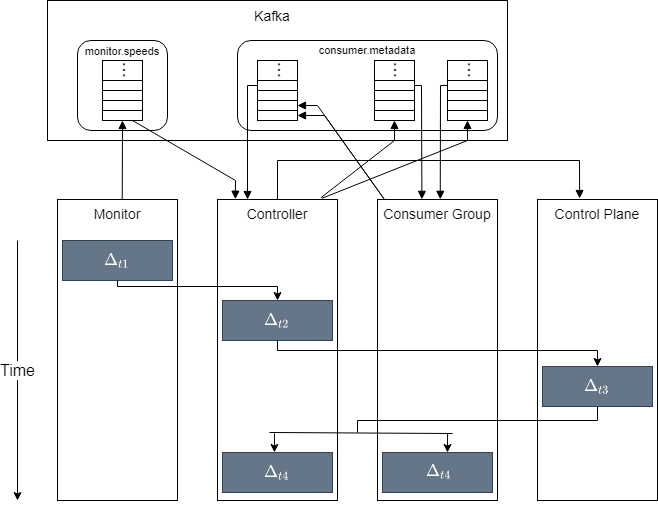
\includegraphics[width=\textwidth]{images/integration/Integration_diagram.png}
\caption{System sequence of events.}
\label{fig:step_event_sequence}
\end{figure}

Initially, a measurement has to be provided by the monitor process to then be
consulted by the controller ($\Delta_{t1}$). The controller then updates the
group's current state based on the new measurement, and proceeds to computing a
new group configuration using one of the heuristic algorithms presented in
Section \ref{subsub:modified_any_fit}.  Having calculated the new configuration,
the controller calculates the difference between the new and current
configuration, to determine the consumers it has to create, the ones it has to
delete, and the messages that have to be communicated to each consumer to reach
the intended state (Section \ref{sub:state_group_management}). This then leads
to the controller communicating with the Kubernetes control plane, to create the
new consumer resources ($\Delta_{t2}$). 

The controller then waits for the newly created deployments to be ready
($\Delta_{t3}$), followed by communicating with the consumer group to inform the
consumers of their change in state, which only terminates as
soon as all messages have been sent out to the respective consumers, and when every message
has been acknowledged back to the controller ($\Delta_{t4}$). This process is illustrated
by Figure \ref{fig:step_event_sequence}.


\section{Monitor Measurement Convergence Time ($\Delta_{t1}$)}
\label{c3sec:MonitorMeasurement}

To evaluate the monitor's response time, the data points were obtained by
feeding the system a step input, similar to what was done in Section
\ref{component:Monitor}, which is obtained by starting a producer that sends
data to one of the partitions the consumer group is consuming data from.

\begin{figure}[H]
\centering
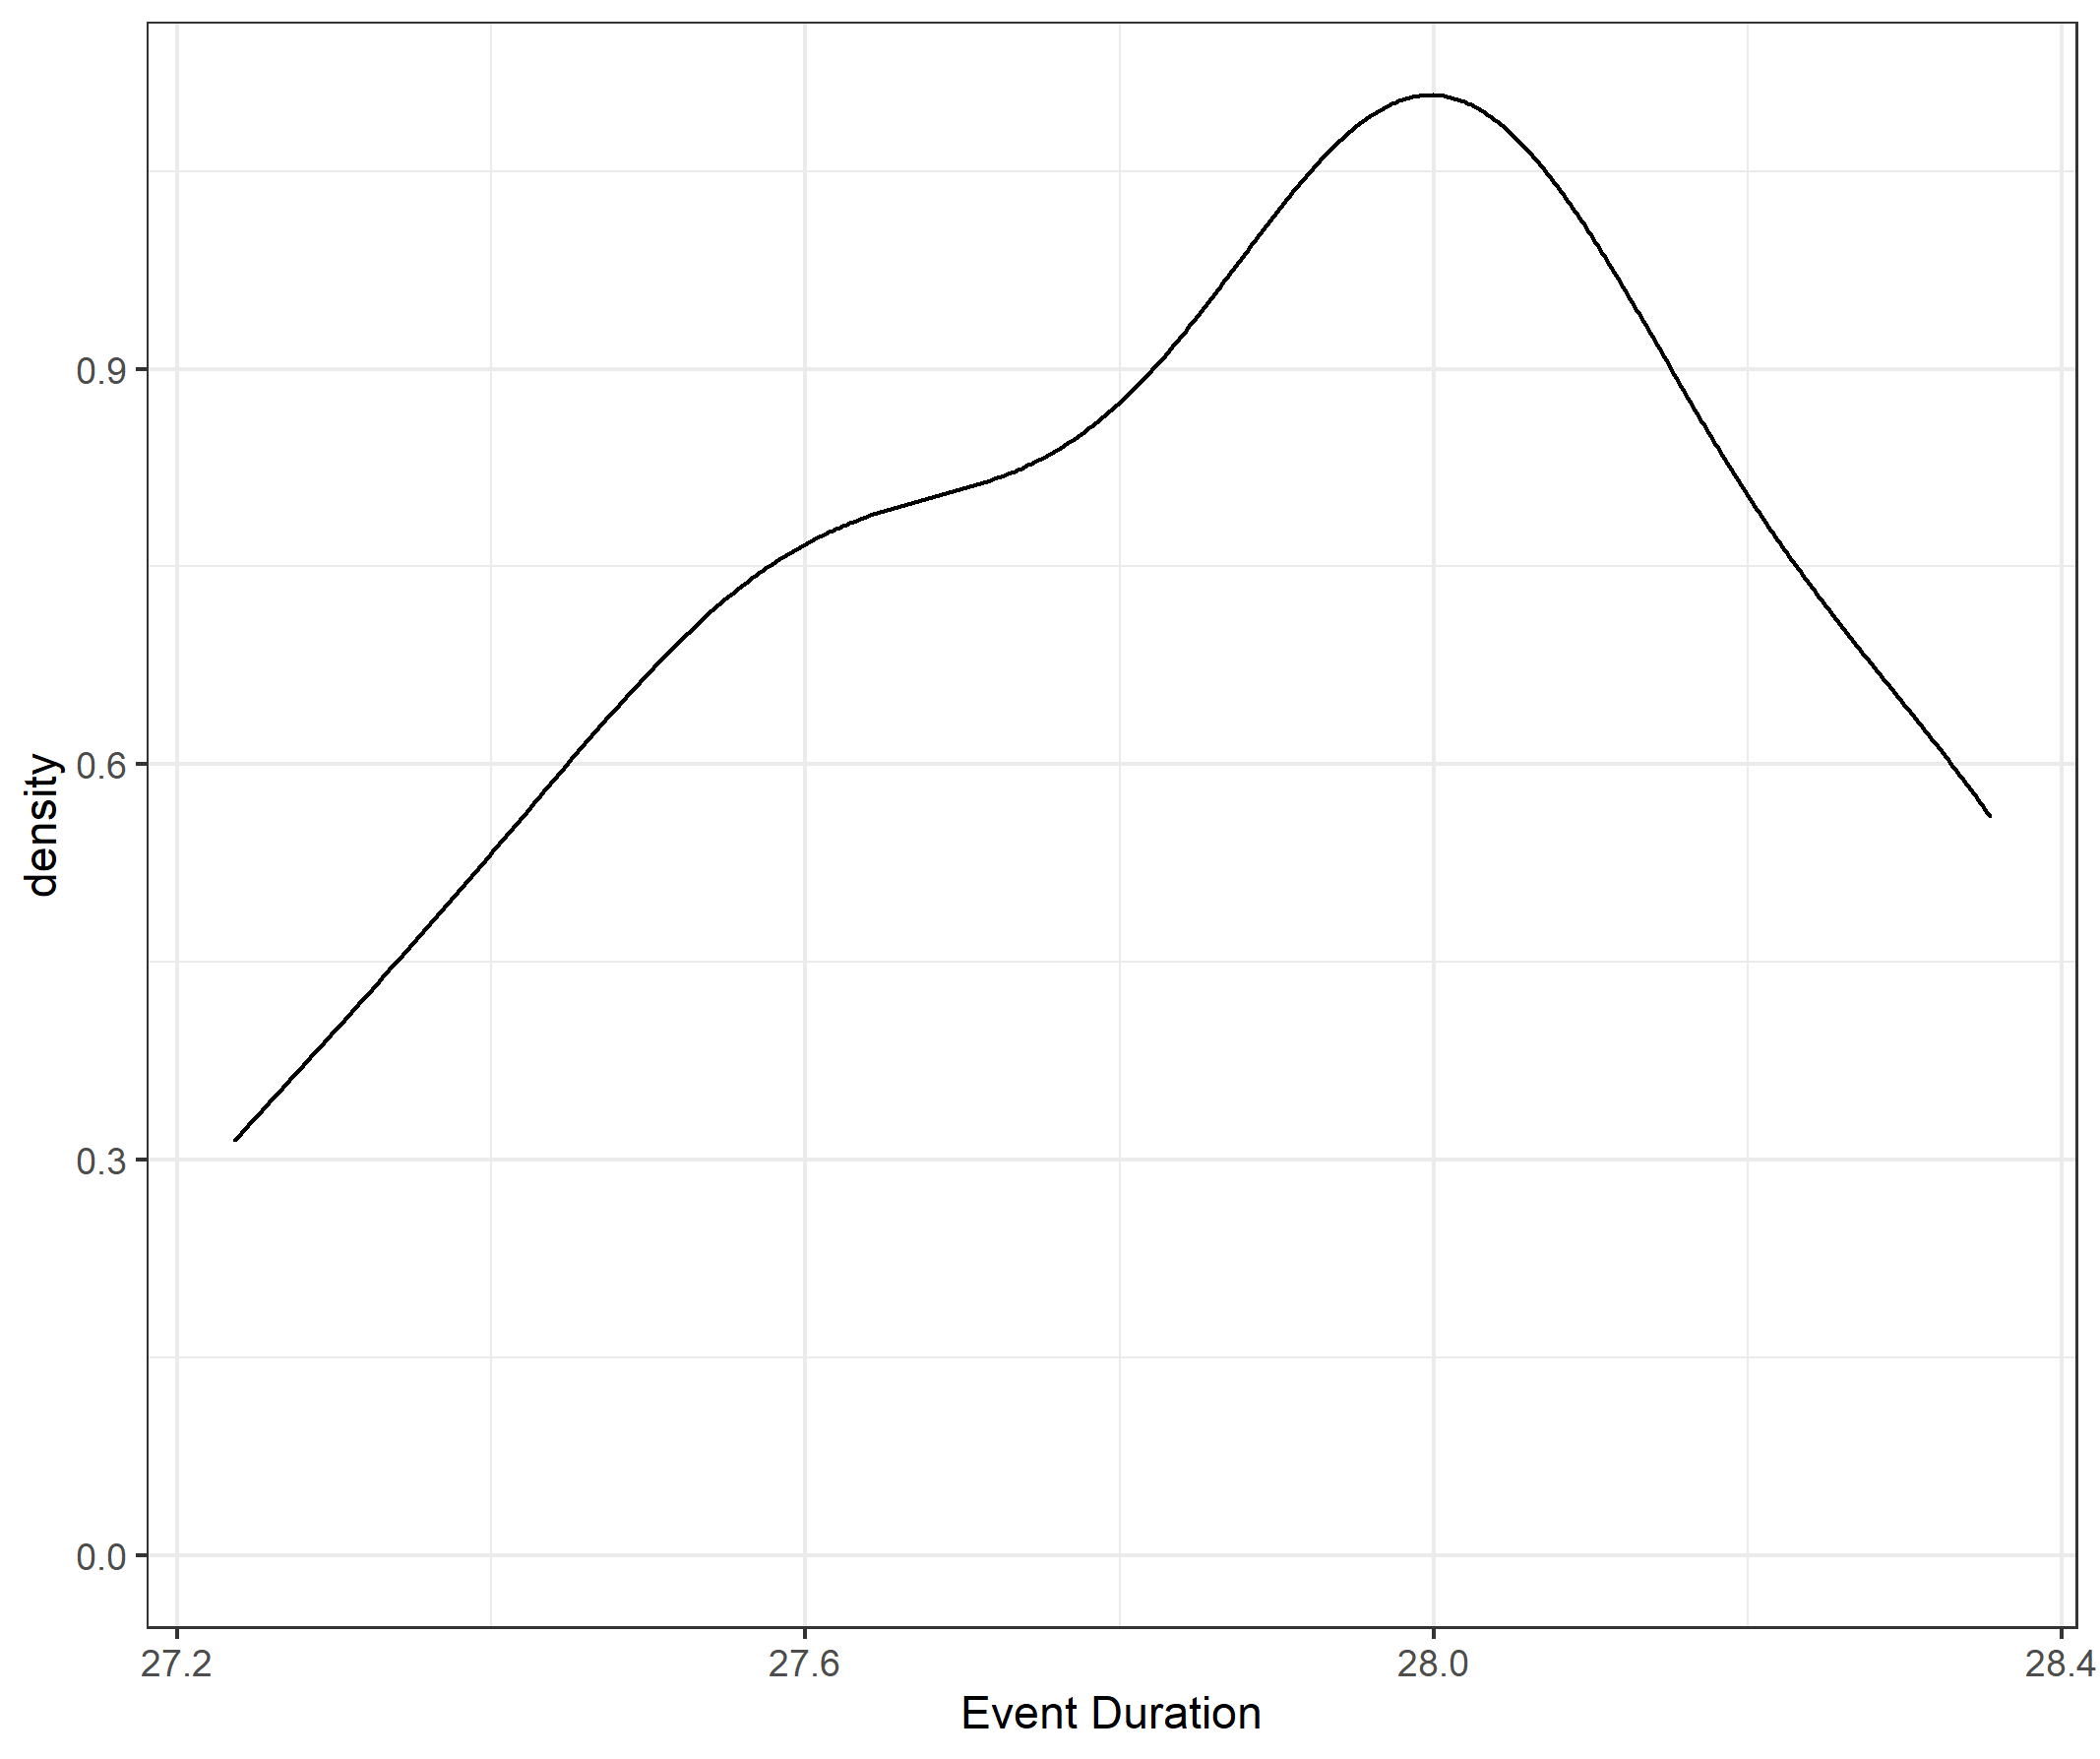
\includegraphics[width=0.6\textwidth]{images/integration/delta1.png}
\caption{
    Distribution of $\Delta_{t1}$ for 31 different step inputs.
}
\label{fig:controller_result_monitor}
\end{figure}

As such, this measure is the time it takes the monitor process to converge to
the real production rate, which, as can be verified in Figure
\ref{fig:controller_result_monitor}, takes no more than $30s$, similar to what
had been obtained in Figure \ref{fig:monitor_step}.

\section{Time to Trigger Scale-up ($\Delta_{t2}$)}

Measured as the time it takes the controller to compute the consumer group's new
assignment, computing the difference between the new and current states, and to
send an asynchronous request to the GKE cluster for every new consumer instance
to be created. To obtain the distribution for this metric, the system was tested
with the aforementioned step inputs and the randomly generated measurement
sequences used in Section \ref{c3subsub:testing}.

\begin{figure}[htb!]
\centering
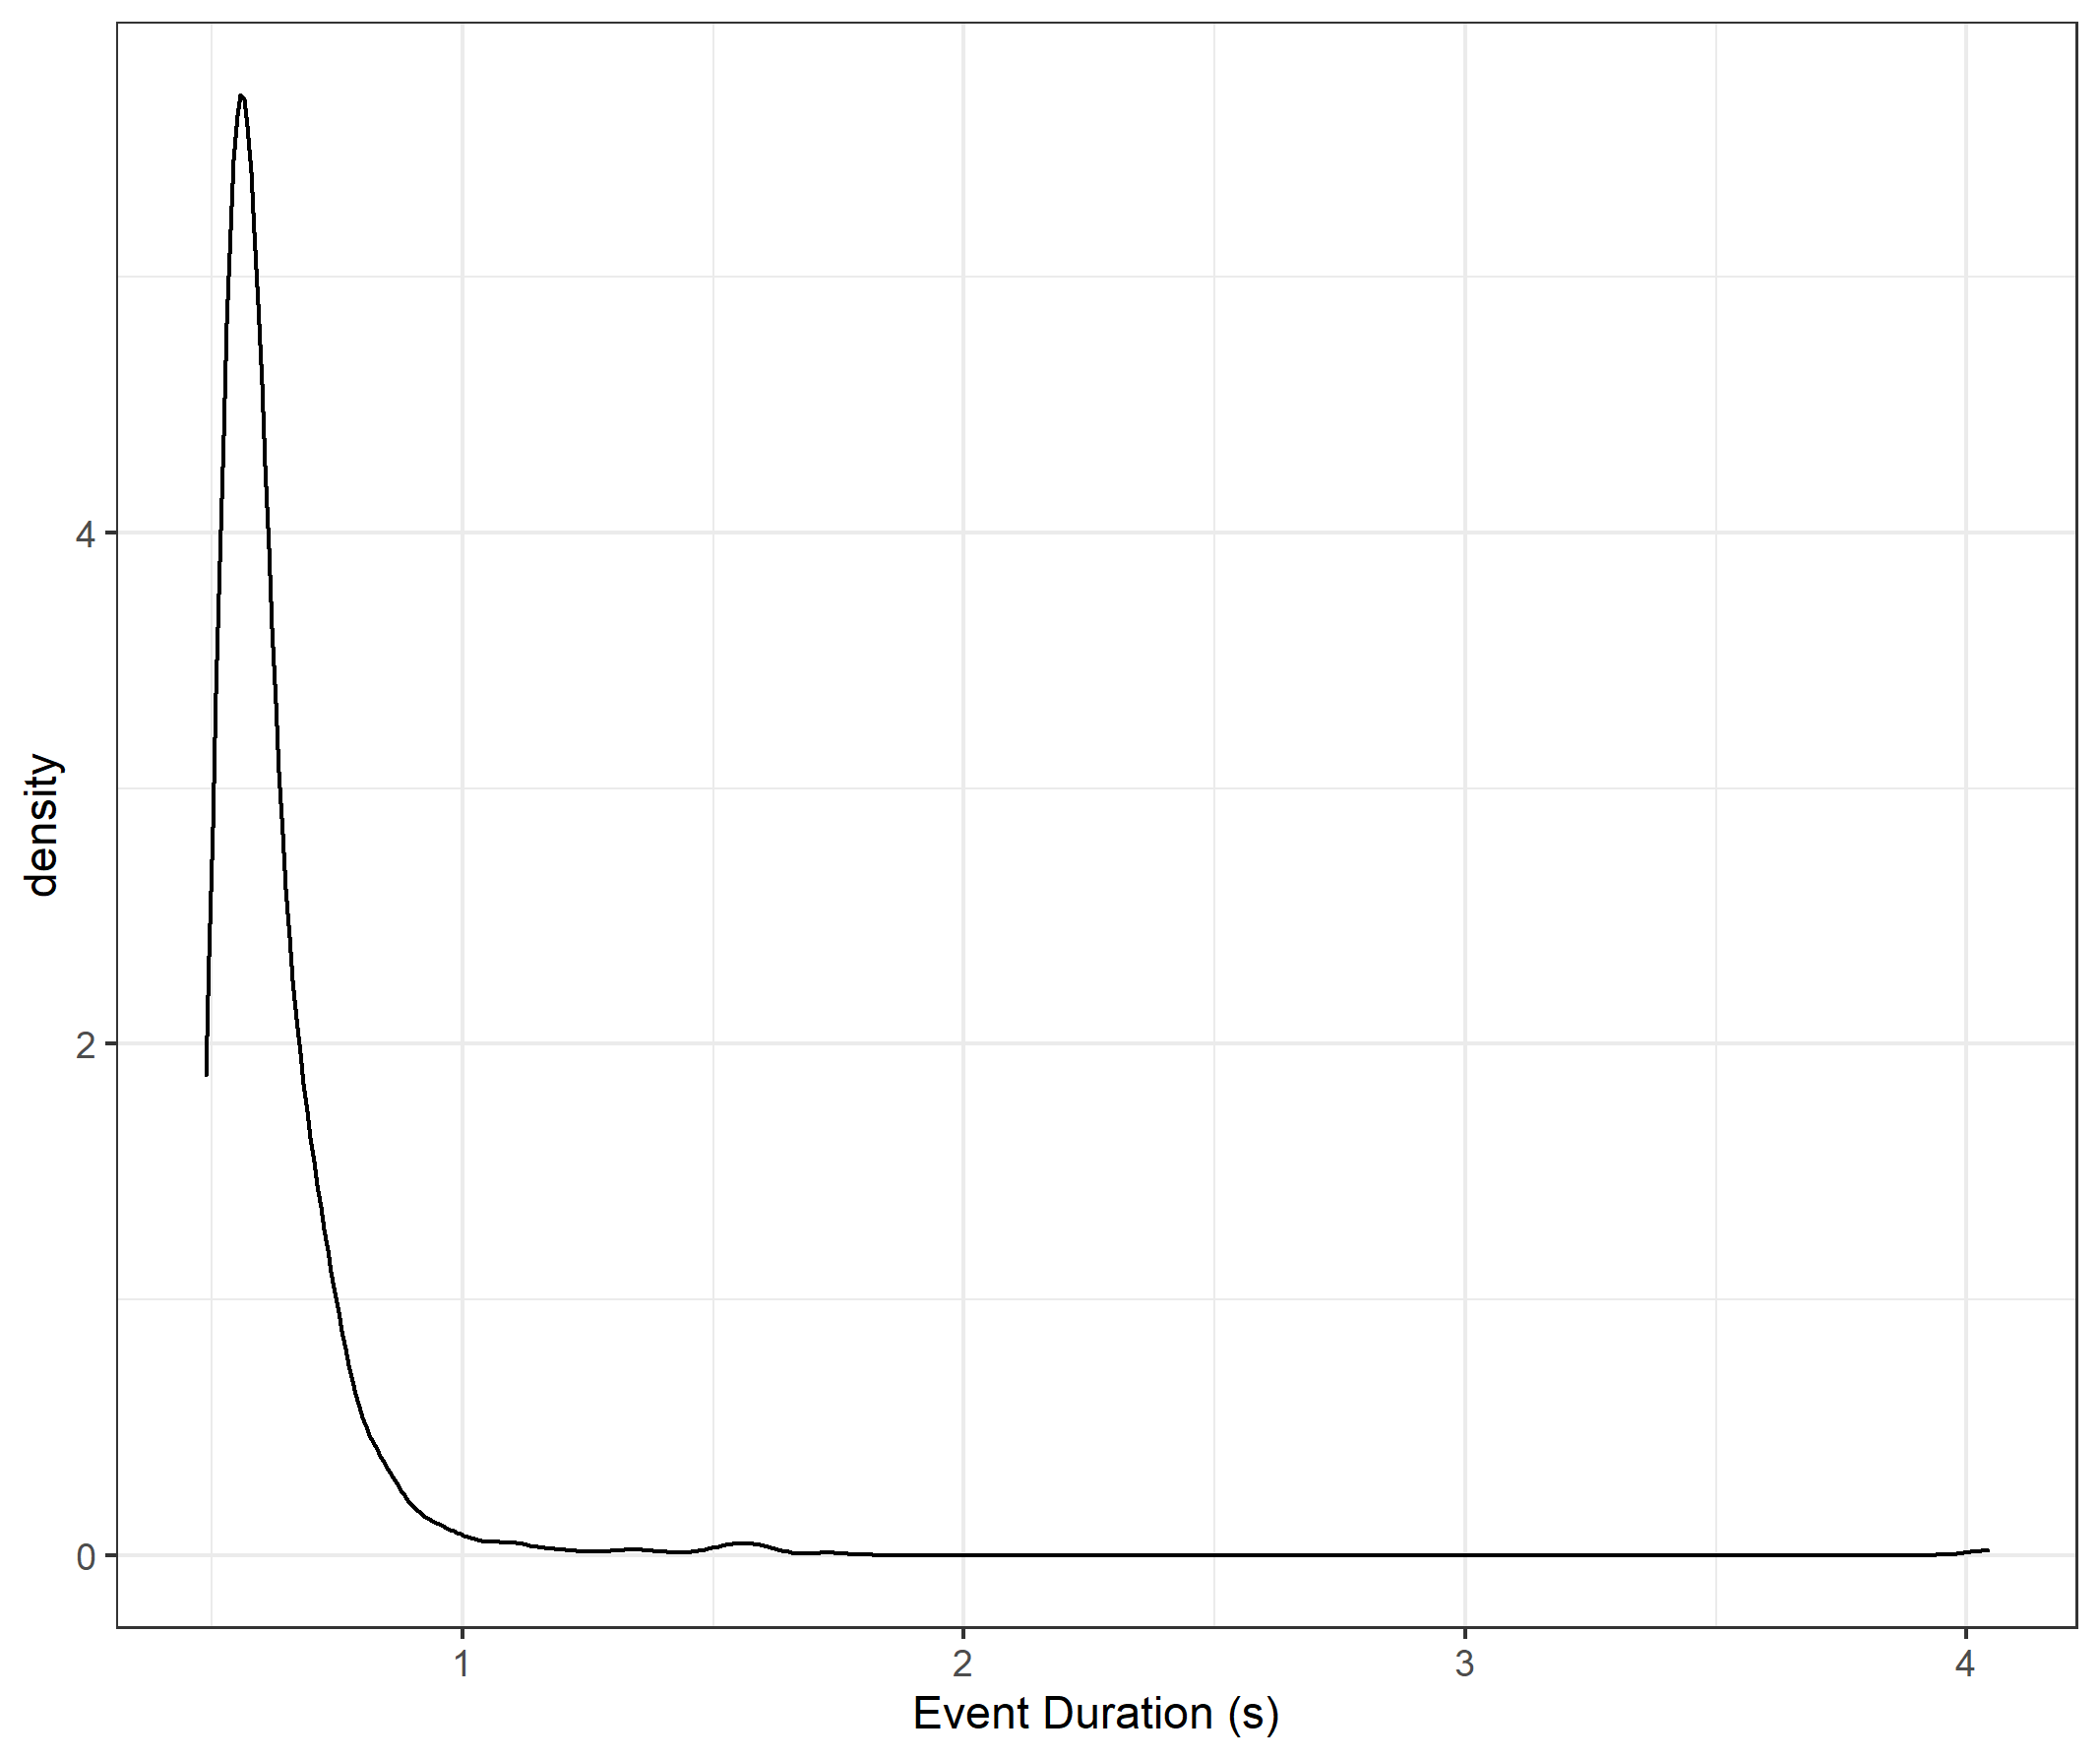
\includegraphics[width=0.6\textwidth]{images/integration/delta2.png}
\caption{
    Distribution of $\Delta_{t2}$ for 1345 observations.
}
\label{fig:controller_result_trigger}
\end{figure}

The time the controller takes with this procedure depends on the number of
partitions to distribute between the consumer group, the algorithm the
controller is executing to figure a new consumer group assignment, and the
number of new consumer instances it has to create in the GKE cluster.

For the tested input data, where there were at most 32 partitions to rebalance
and no more than 20 consumers to be created in a single interation, the event
consistently takes less than 1 second to be executed as shown in Figure
\ref{fig:controller_result_trigger}.

\section{Newly Created Deployments Ready ($\Delta_{t3}$)}

After making the asynchronous request to the GKE cluster, the control plane
schedules the pods to a node, and within the node starts the containers that are
to be executed.

\begin{figure}[htb!]
\centering
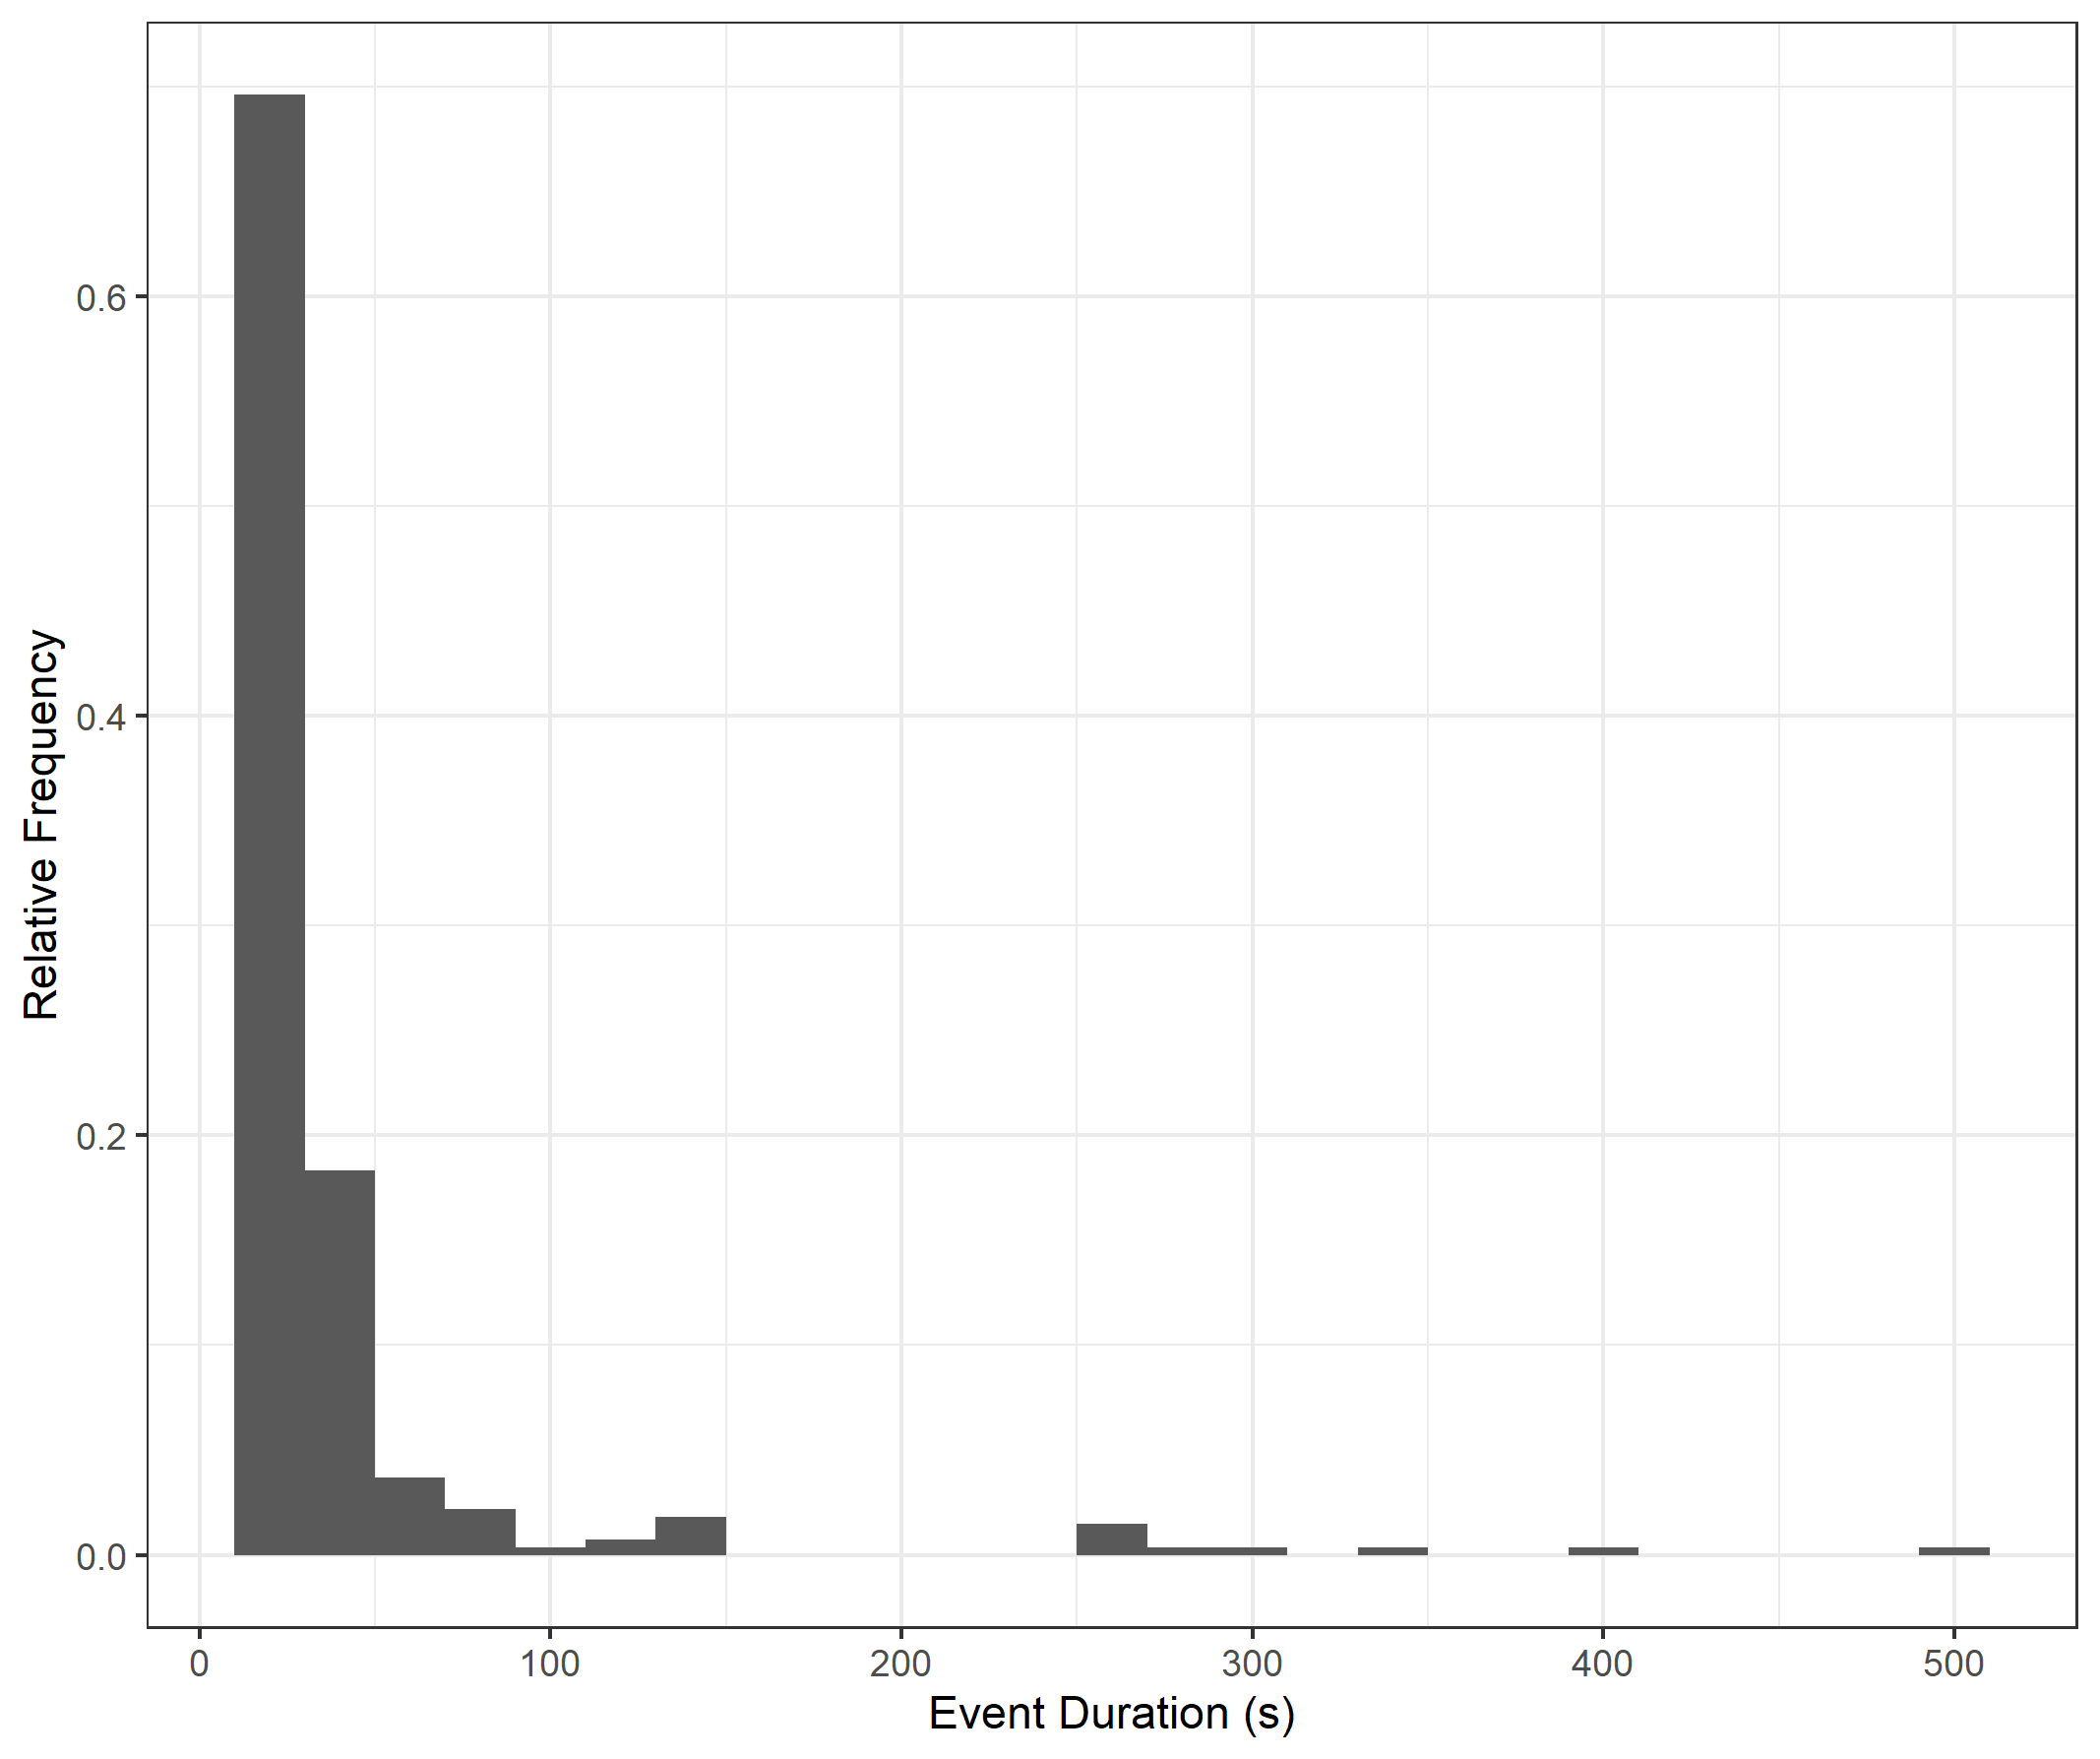
\includegraphics[width=0.6\textwidth]{images/integration/delta3.png}
\caption{
    Histogram of $\Delta_{t3}$ for 273 observations.
}
\label{fig:controller_result_kubernetes}
\end{figure}

After discarding the data points that didn't have the controller creating any
new consumer, there remain 273 data points, which show two clusters of data
points that are justified by two different scenarios when creating a new pod. 

The first, and most frequent (88\%), has the GKE cluster taking between $[10,
50]$ seconds to have a new consumer instance ready. This is usually the case when the
controller requests for the creation of new consumer instances and the
Kubernetes cluster has resources available to schedule the new consumer
instance. As such, the event's duration is related to the time it takes the
scheduled node(s) to download the image from the container registry, and to
start the containers.

The second group of data points, any time span greater than $50s$ (represents
12\% of the data points), occurs when the Kubernetes cluster does not have any
available resources. Here the actions the cluster undergoes are adding a new
node to the cluster, and only then scheduling the consumer instance into the new
available node. Due to the autoscaling feature of the GKE cluster, this is done
automatically but it is also more inconsistent, having data points taking up to
$500s$, although very sporadically.

Although there isn't much control over the time it takes the Kubernetes cluster
to schedule and start the pods, one variable that can be controlled is the size
of the image which has to be downloaded by the nodes that were assigned the
newly created consumer instances.

\section{Communicating Change in State ($\Delta_{t4}$)}

Each partition that the controller is monitoring can either be associated with a
start, stop, rebalance or a do nothing action. A start action refers to the case
where there is no consumer currently consuming data from the partition, and the
controller has assigned that partition to a consumer in its newly computed
consumer group state. The stop action occurs when the controller no longer wants
a consumer assigned to this partition therefore having no consumer fetching data
from this partition in the group's future state. Rebalancing happens when the
controller is changing the partition from being assigned from one consumer to
another. Lastly, as the name suggests, do nothing is when there are no actions to
be communicated for a partition. 

Since there is no concurrent read from the partition when the controller is
analyzing a start or a stop action, the controller can send this message as soon
as it enters this event, having to wait at most for one consumer cycle to receive
the acknowledgement by the consumer. 

When rebalancing, the controller has to first send out the stop command, wait
for a response, send out the start command, and wait for the response. Without
taking into account any processing and network delays, at worst, the controller
might have to wait for 2 consumer cycles to be able to rebalance a partition.

\begin{figure}[htb!]
\centering
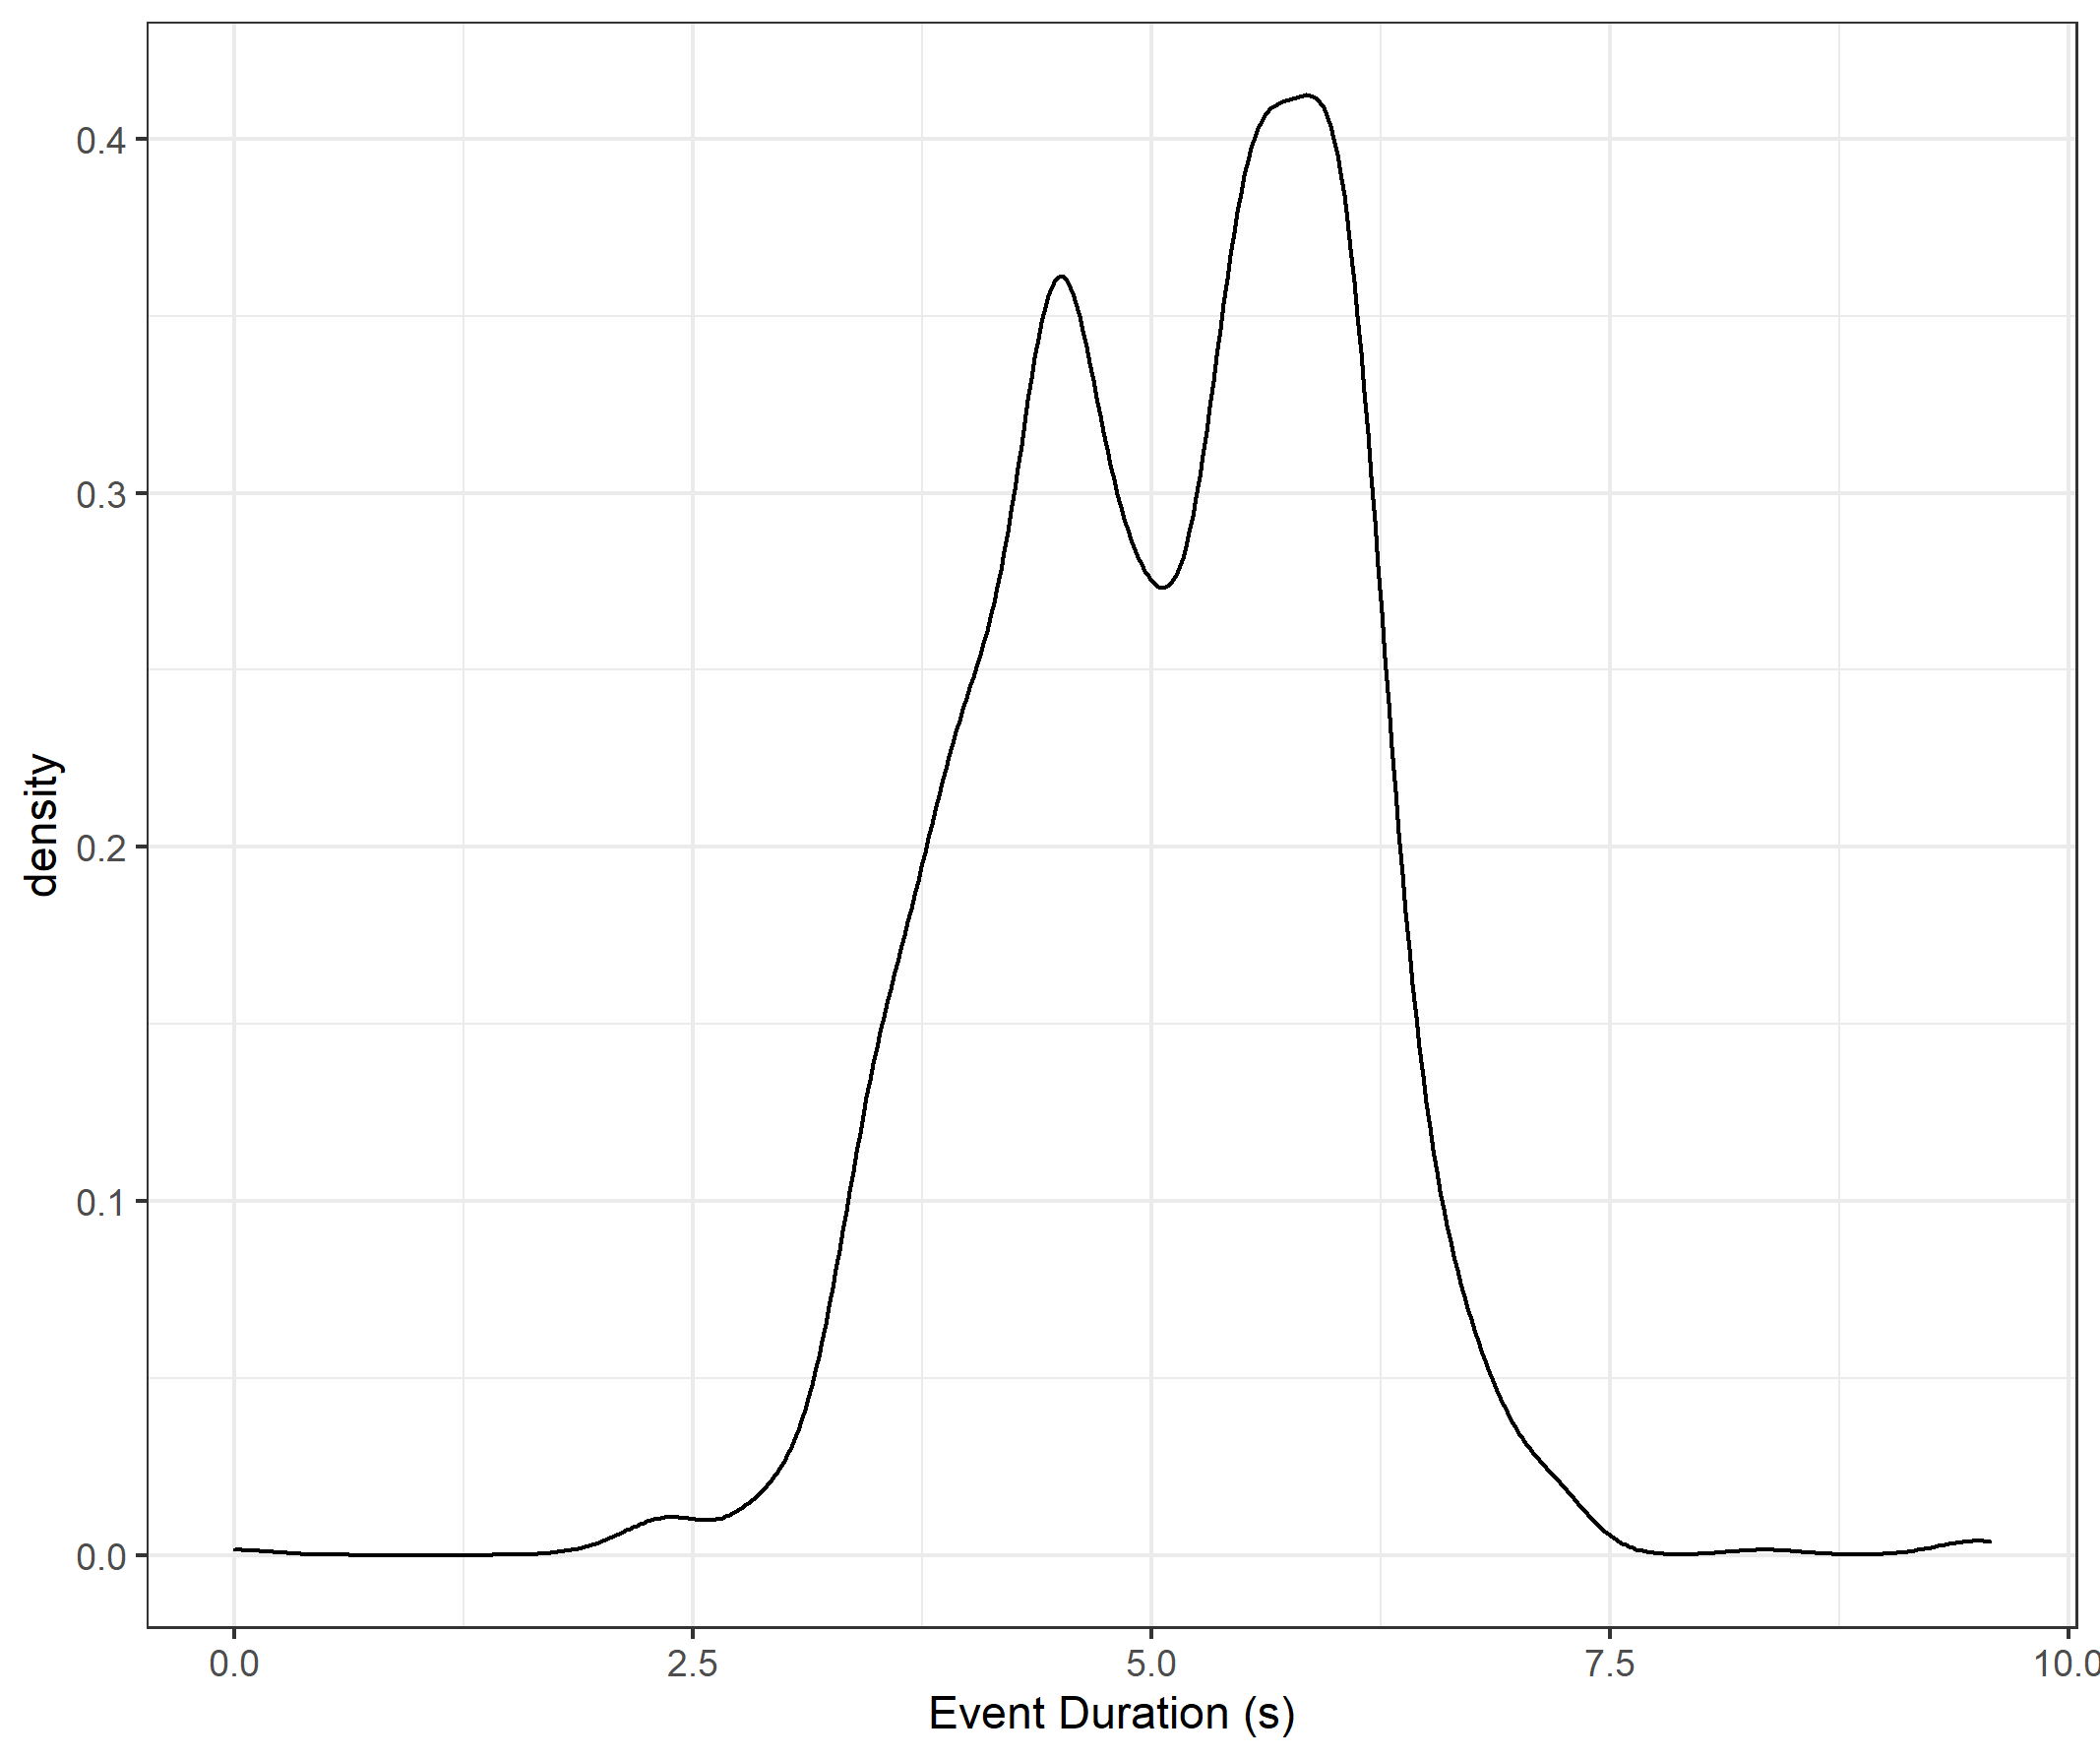
\includegraphics[width=0.6\textwidth]{images/integration/delta4.png}
\caption{
    Distribution of $\Delta_{t4}$ for 1331 observations.
}
\label{fig:controller_result_change_state}
\end{figure}

A consumer's insert cycle goes through the different phases mentioned in Section
\ref{component:consumer}, and only after performing it's tasks does it verify
the metadata queue to check if it has received any change in state command. For
this reason, between two metadata reads from the \lstinline{consumer.metadata}
topic, it takes the consumer one whole insert cycle. Having defined in Section
\ref{c3subsub:consumer_maximum_capacity} that the consumer gathers at most
$5Mbytes$ per cycle, and provided the results from Figure
\ref{fig:consumer_capacity}, which indicate the consumer has a data rate of
approximately $2Mbytes/s$, each consumer cycle can take approximately $2.5s$.
Since the controller has to wait for two consumer cycles, this would imply that
changing the group's state could take around 5 seconds, as can be seen in Figure
\ref{fig:controller_result_change_state}

It is also worth noting that the more consumers there are in the group, the
higher the probability that the controller has to wait 1 whole cycle after
sending out the stop command, and another whole cycle after a start command, as
the communication is performed with more consumers.

Although this analysis was performed for a single partition, without any loss of
generality and due to the fact that the controller sends out the change state
commands in batch, the time it takes the controller to change a consumer group's
state remains at 2 consumer cycles.

To vary the duration of this event, the consumer's cycle has to be altered using
the \lstinline{BATCH_BYTES} and \lstinline{WAIT_TIME_SECS} parameters, which in
turn have an effect on the time the consumer spends in a whole insert cycle.

\chapter{Conclusion and Future Work} 
\label{chap:conclusions}

\section{Summary and Discussion of Thesis Results}

The work developed in this thesis challenges the existing methods used to scale a Kafka consumer group and how the load should be distributed between the various consumers.

The goal was to deterministically solve the autoscaling problem related to a group of consumers, which in turn was modeled as a Bin Packing Problem where the items that have to be assigned a bin can change in size over time. Due to this particular feature, a new metric was introduced to determine a rebalance score (Rscore) for a given iteration. 

The Rscore introduced a new concern when executing an algorithm to solve the bin packing problem, and for this reason 4 new algorithms were presented to heuristically solve the BPP, while at the same time taking into consideration how the items (partitions) were rebalanced to different bins (consumers). Three of the presented algorithms (MWF, MBFP and MBF), proved themselves to be a competitive alternative, consistently belonging to the pareto front \ref{fig:pareto_front} when comparing the multi-variate optimization with regards to the number of consumers and the Rscore.

To further consolidate the BPP Model, the consumer was tested in diverse conditions to determine whether a constant bin size model could be used for the scenario at hand. Provided the results in \ref{result:bin capacity}, the BPP was then modeled as its single bin size variant.

The different parts in the system interacted with one another as expected to deliver an autoscaling consumer group capable of adapting depending on the current load of the system as shown in \ref{c4}.

\section{Future Work}

Given the multiple parts developed within this system, there is a lot of room for improvement. Most notably, due to the close relationship between the system and the Kubernetes cluster, the autoscaler could be wrapped as a Kubernetes Operator \cite{KuberenetesOperator} as is common with systems of this kind (\cite{Kubegres, PulumiOperator, KEDA}).

\subsection{Monitor}

To the best of my knowledge, for lack of a better metric being provided by the Kafka cluster, the value that was used to track the write speed of each partition was the number of bytes in each partition. For this reason, a process \ref{component:Monitor} was used to evaluate the speed of each partition by historically storing the amount of bytes in a partition at a certain timestamp.

A clear disadvantage of using this component is the fact that if \lstinline[language=Python]{retention.ms != -1}, this means a record is deleted from its partition after \lstinline[language=Python]{retention.ms} which leads to a reduction in the amount of bytes in the partition. The monitor process (\ref{component:Monitor}) then erroneously evaluates a negative partition write speed. To circumvent this behaviour, either one of the following metrics provided by Kafka would suffice: The current write speed (bytes/s) per partition; A historic amount of bytes that have been written to a partition.

Since the monitor process presents the write speed as the average data rate over the last 30 seconds, using a different strategy to evaluate the speed could lead to more robust measures.

\subsection{Consumer}

If the network is experiencing increased latency, the current implementation of the autoscaler does not account for changes in the size of the consumer capacity, therefore the controller assumes a maximum capacity of a consumer which is not accurate within this scenario. Metrics related to a consumer's performance provided by Kafka JMX metrics could be leveraged to obtain a more accurate dynamic representation of the consumer's current capacity. This could also lead to a variable bin size BPP.

\subsection{Controller}

Throughout this thesis, the controller process was presented with strict execution rules and actions to manage the Kafka consumer group. Evolving this component into a more abstract concept, could not only maintain its current functionalities, but it could also be used to more accurately solve load balancing within a consumer group without necessarily modeling the problem as a BPP. 

In fact, the heuristic algorithms that make use of the worst fit rule when assigning partitions to consumers, are at the same time applying a load balancer rule between the available consumers.

\section{Final Remarks}

In spite of the fact that, as a whole, the thesis presents quite a specific use case, individually several of Kafka's functionalities are challenged and tested alternatives are also provided which can be used as a foundation so as to improve the way in which a consumer's load is modeled, and the manner in which the load is distributed between the elements of a consumer group.


%% Comment next 2 commands if numbered appendices are not used
\appendix
\chapter{CellTAN Development}

\section{Statistical tests for measure of association} \label{ap1:stats}

\subsection{Pearson's chi squared test} \label{ap1:pearsonschi}

\begin{equation}
    \chi^2 = \sum_{i=1}^{k} \frac{(O_i - E_i)^2}{E_i}
\end{equation}
    
where:
\begin{align*}
\chi^2 & : \text{Chi-squared statistic} \\
O_i & : \text{Observed frequency for category } i \\
E_i & : \text{Expected frequency for category } i \\
k & : \text{Number of categories or cells in the data}
\end{align*}


\subsection{Fischer's exact test} \label{ap1:fischer}

\begin{equation}
    p = \frac{{\binom{a}{x} \binom{b}{y}}}{{\binom{N}{n}}}
\end{equation}

where:
\begin{align*}
    p & : \text{p-value of the test} \\
    a & : \text{Number of successes in group A} \\
    b & : \text{Number of successes in group B} \\
    x & : \text{Number of successes of interest in group A} \\
    y & : \text{Number of successes of interest in group B} \\
    N & : \text{Total number of observations} \\
    n & : \text{Number of observations in group A}
\end{align*}


\subsection{Odds ratio} \label{ap1:oddsratio}

\begin{equation}
OR = \frac{{a \cdot d}}{{b \cdot c}}
\end{equation}

where:
\begin{align*}
OR & : \text{Odds ratio} \\
a & : \text{Number of successes in group A} \\
b & : \text{Number of failures in group A} \\
c & : \text{Number of successes in group B} \\
d & : \text{Number of failures in group B}
\end{align*}

\subsection{Phi coefficient} \label{ap1:phi}

\begin{equation}
\phi = \sqrt{\frac{\chi^2}{N}}
\end{equation}

where:
\begin{align*}
\phi & : \text{Phi coefficient} \\
\chi^2 & : \text{Chi-squared statistic} \\
N & : \text{Total number of observations}
\end{align*}

\subsection{Contingency coefficient C} \label{ap1:contingencyc}

\begin{equation}
C = \sqrt{\frac{\chi^2}{N + \chi^2}}
\end{equation}

where:
\begin{align*}
C & : \text{Contigency coefficient} \\
\chi^2 & : \text{Chi-squared statistic} \\
N & : \text{Total number of observations}
\end{align*}


\subsection{Theil's U} \label{ap1:theilsu}

\begin{equation}
U(x|y) = \frac{H(x) - H(x|y)}{H(x)}
\end{equation}

Entropy of variable x:
\begin{equation}
H(x) = -\sum_{i=1}^{n} p(x_i) \log(p(x_i))
\end{equation}

Conditional entropy of variable x given variable y:
\begin{equation}
H(x|y) = -\sum_{i=1}^{n} \sum_{j=1}^{m} p(x_i, y_j) \log\left(\frac{p(x_i, y_j)}{p(y_j)}\right)
\end{equation}


\section{Technology stack} \label{ap1:techstack}

\begin{figure}[h!]
    \centering
    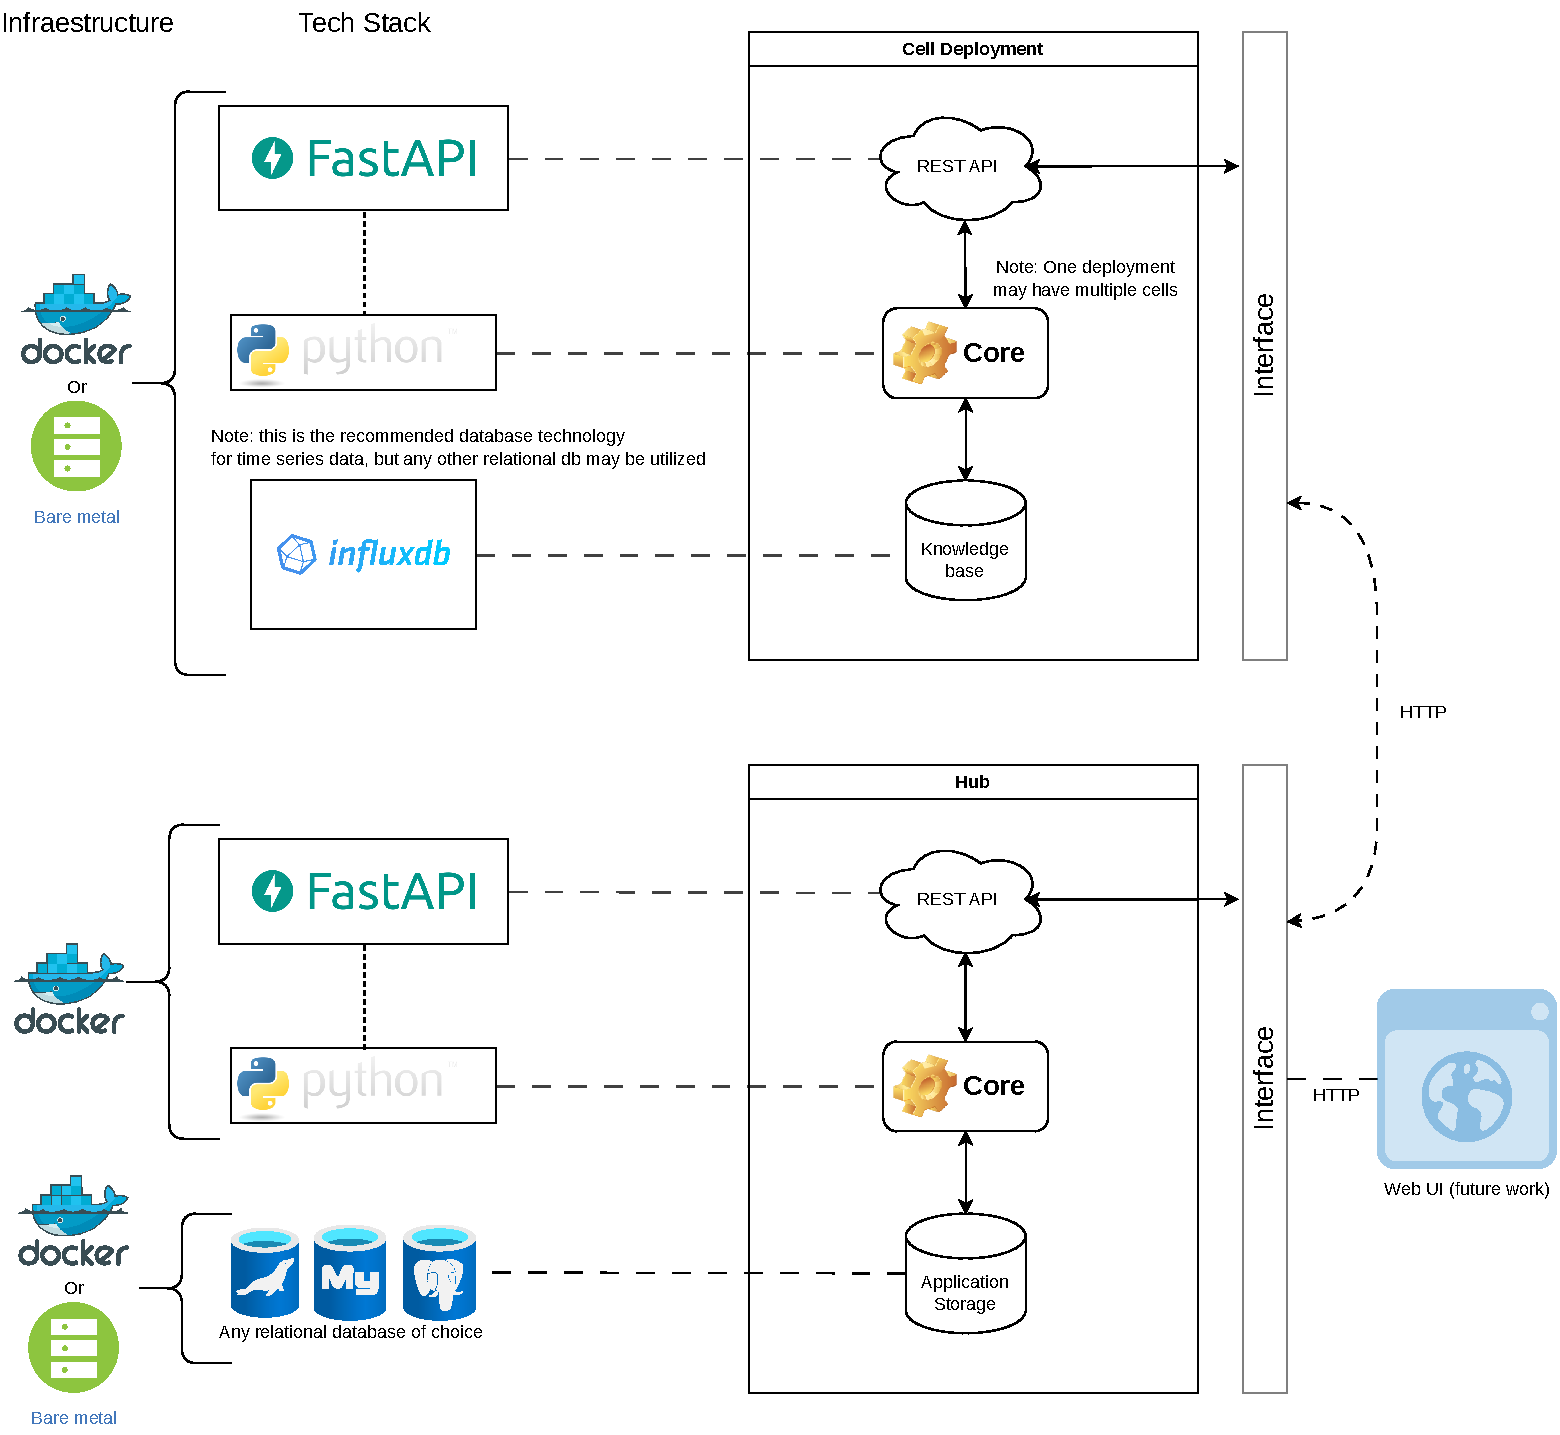
\includegraphics[width=\linewidth]{figures/appendix/a_development/techstack.pdf}
    \caption{Technology stack of the Cell and Hub of CellTAN.}
    \label{fig:techstack}
\end{figure}


\section{Cell configuration} \label{ap1:config}
 
% TODO overview da configuração da célula e ficheiro de configuração


\printbibliography

%% Index
%% Uncomment next command if index is required, 
%% don't forget to run ``makeindex tese'' command
%\PrintIndex
\end{document}
